\documentclass[sigconf]{acmart}

\usepackage{booktabs} 

\usepackage{amsmath}
\usepackage[linesnumbered,boxed]{algorithm2e}
\usepackage{subfigure}
\usepackage{epstopdf}
\usepackage{graphicx}
\usepackage{color}
\usepackage{multirow}
\usepackage{colortbl}
\definecolor{pink}{RGB}{240,128,128}

\newenvironment{shrinkeq}[1]
{ \bgroup
  \addtolength\abovedisplayshortskip{#1}
  \addtolength\abovedisplayskip{#1}
  \addtolength\belowdisplayshortskip{#1}
  \addtolength\belowdisplayskip{#1}}
{\egroup\ignorespacesafterend}



\setcopyright{none}

\begin{document}
\title{The Spiral of Silence and Its Application in Recommender Systems}
\author{Paper 1457}


\begin{abstract}
Are people in recommender systems less willing to speak out if they perceive they are in the minority? We verify the famous ``spiral of silence'' theory in real recommender systems. We study the trend of holding back opinions over time. We discuss the impact of opinion leaders and peer groups on users' perceptions of the opinion climate. We confirm the consistency of hardcore users and that hardcore is related to attitude certainty, personal interest, item popularity and moral basis. The phenomenon of silent minority harms the performance of conventional recommender systems. We propose novel models which assume that the probability a user willing to express opinion is dependent on the rating and how the rating is divergent from the perceived opinion climate. Furthermore, we utilize our empirical discoveries to guide the building of recommender models. We model the formation of community, opinion leaders, hardcore personality and item popularity to enhance recommendation performance.  Experimental results demonstrate that our models  outperform state-of-the-art recommendation models.
  

\end{abstract}


\keywords{Spiral of Silence, Missing not at Random, Recommender System}

\maketitle
\section{Introduction}\label{sec:introduction}
%The theory

In 1974, German political scientist Elisabeth Noelle-Neumann proposed the Spiral of Silence Theory\footnote{In the remaining of this paper, the Spiral of Silence theory will be referred as ``the theory''.}~\cite{Neolle-Neumann1993spiral}. The theory states that, due to the ``fear of isolation'', people are less willing to express their opinions if they perceive that they are not supported by the majority. It results in a spiral process in which the majority opinion receives growing popularity while other opinions are gradually pushed back. The process continues until the majority opinion ultimately becomes a social norm.

%Related Empirical Study
The theory has been acknowledged as ``one of the most influential recent theories of public opinion formation''~\cite{Kennamer1990Self}. In the literature of mass communication and political science, many studies testify the theory. Typically, they conduct surveys and ask subjects to rate the willingness to speak out (i.e. enter a conversation, vote, donate, etc.) if their opinions are in the minority. However, this type of experiment protocols may be problematic, because the findings are based on hypothetical willingness instead of actual willingness~\cite{Carroll1997Perceived}. The theory in its online form also triggers considerable critiques. Some researchers point out that, within the online context, factors such as anonymity might decrease the fear of isolation and thus empower ``people in the minority to speak up more''~\cite{mcdevitt2003spiral}.

%Contribution: Empirical Study, discoveries
Our first contribution in this work is to empirically verify the theory in terms of actual willingness to speak out in \textbf{R}ecommender \textbf{S}ystems (RS). We use several real data sets to analyze response and its pattern over time, given how the users' opinions diverge from the perceived ``opinion climate''. The increasing trend in the portion of majority opinion is confirmed by Mann-Kendall trend test. 

We then further examine some key components in the theory. The key components include: (1) The perceptron of ``opinion climate''. The theory asserts that people use their ``quasi-statistical'' sense to assess current majority opinion. Our results reveal that, assessment of ``opinion climate'' might be related to the opinion leaders and the ``peer group'' of people with similar interests. (2) The existence of ``hardcore users''. The theory presumes that some people (``hardcore users'') are more active while the rest are more reluctant to respond. We empirically verify the existence of a consistent hardcore group. Furthermore, hardcore users tend to choose more extreme rating values. (3) The strategies to remain silent. The theory presumes that users might choose different strategies to remain silent according to the nature of items. We observe that, item's popularity, personal interest and moral basis have significant impacts on the response patterns. Users are more prone to speak out for popular items, items that are not important to them, and to praise a criticized item than to criticize an appreciated item.


%Challenge to RS
The phenomenon of ``silent minority'' will harm the performance of RS. Fig.~\ref{fig:example} gives an illustrative example. Suppose \emph{Alice} is a sensitive user who only responds to items on which she agrees with the majority. Given her responses, a conventional recommender will estimate her preferences as the average user preference. For example, a collaborative filtering recommender will determine \emph{Alice}'s nearest neighbor as \emph{Bob} and \emph{Clare}, because their rating similarities are the highest. It leads to a predicted rating $5$ for \emph{Alice} on \emph{Aliens}. As we can see from the example, the prediction is severely biased.

%running example
\begin{figure}
\centering
\small
\begin{tabular}{|c|c|c|c|c|c|}
\hline
 & Aliens &  Ben-Hur  & Casino & Dangal & Eskiya \\\hline\hline
 Alice &\emph{ (2)} & 3 & & 3 &  \\\hline
 Bob & 5 & 3 & & 3 &2 \\\hline
Clare & 5 & 3 &5 & 3 & \\\hline
 Diane &  &  &2 & 3 & 4 \\\hline
 Elle & 5 &  &2 &  &  1\\\hline
\end{tabular}
\caption{A toy example of 5 users's ratings on 5 movies, ``hidden'' opinions are printed in italic within parenthesis}\label{fig:example}
\end{figure}

%Related Work
To address the challenge of ``spiral of silence'', one needs to model the missing ratings as \textbf{M}issing \textbf{N}ot \textbf{A}t \textbf{R}andom observations(MNAR). In the RS community,  MNAR models explicitly generate user responses by user ratings~\cite{Hernandez-Lobato2014Probabilistic,Steck2010Training,Marlin2009Collaborative}. Instead of optimizing $p(R|\Theta)$, which is the likelihood of ratings, MNAR models optimize $p(R,X|\Theta)$, where $X$ is the set of \textit{response} variables indicating whether a rating is missing. Consequently, MNAR models achieve better performance in predicting both ratings and responses.

%Contribution
In the nutshell, our models fall in the MNAR framework. However, for the best of our knowledge, we are the first to apply ``spiral of silence'' theory in recommender systems and consider the perception of support as a factor in an MNAR model. We model the possibility of user ``speaking out'' as dependent on users' perception of opinion climate.  Our model adjusts the bias of response probability by connecting the rating values and opinion climate, thus improves the performances of traditional MNAR models, which are solely based on rating values.  In the experiments on real data sets, our model achieves best results ($NDCG@5$ 0.79) compared with other state-of-the-art MNAR models(best $NDCG@5$ 0.7).

We also utilize the findings in our empirical study to build variant models. We incorporate hidden community, hardcore persona and item specific factors into the model. The comparative performances of model variants support the discoveries about the impact of social identity, hardcore groups and silent strategy on self definition of minority. We believe our study sheds insights into bridging social science and computer engineering.

%paper structure
The paper is organized as follows. In Sec~\ref{sec:related} we briefly introduce the related works. In Sec~\ref{sec:empirical} we present our empirical study on several real data sets. In Sec~\ref{sec:model} we propose several model variants, based on the findings in Sec.~\ref{sec:empirical}. In Sec.~\ref{sec:experiment} we demonstrate and analyze comparative performances of the models. Finally, in Sec.~\ref{sec:conclusion} we conclude our contribution and look into the future work.


\section{Related Work}\label{sec:related}
%recommender systems: collaborative filtering
Recently, recommendation system has attracted a lot of research attentions. In the fruitful literature, matrix factorization~\cite{Koren2009Matrix} techniques have exhibited superior performances in rating predictions. Probabilistic matrix factorization~\cite{salakhutdinov2008probabilistic} implements the idea of matrix factorization from a probabilistic generative perspective. Opinion leaders and social communities can be included in this framework. For example, a SVD style model~\cite{Liu2011Wisdom} factorizes the rating matrix to most representative users. The social recommender~\cite{Jamali2011Generalized} models how a user's rating is affected by his/her trusted friends in a community.

%MNAR

When data is not missing at random, the probability of generating both observations and missing ratings (thus the ``whole'' data set) is not proportional to the likelihood of observed ratings. Marline et.al presented a pioneer work of Missing Not At Random (MNAR) models~\cite{Marlin2009Collaborative}. It assumes that response is a binary variable, which is generated by a Bernoulli distribution associated with the rating value. Along this line, several successive research works introduce new mechanism to generate responses from ratings. A continuous rating is allowed in ~\cite{Ling2012Response} with a step function. Such a soft assignment model is further improved in ~\cite{Yang2015Boosting} with a mini batch algorithm. An OR operation~\cite{Kim2014Bayesian} is adopted over per-item, per-user, per-rating-value parameters. The most complicated model is given by ~\cite{Hernandez-Lobato2014Probabilistic}, which proposes seperate generative processes for the complete ratings and the responses, and cover the rating matrix by the response matrix as a mask to form the observations.

Another line is to consider a semi-observed variable ``exposure''. The response is determined by whether the item is exposed to the user, as well as the potential rating. A few recent works~\cite{Liang2016Modeling,Gopalan2015Scalable} fall into this category. Instead of directly producing a response based on the hidden rating, an alternative approach is to probabilistically relate responses and ratings. For example, ~\cite{Ohsawa2016Gated} presumes a parameter is involved in both processes of generating ratings and responses. 

%dynamics of public opinion
A long and refreshing research topic is to study the dynamics of public opinion. Many empirical studies are performed in various domains. Some researchers have observed the trend of increasing average ratings. They offered several explanations. The first one is selection bias: users select and rate entities they are likely to like~\cite{Dalvi2013Para}. The second hypothesis is choice-supportive bias~\cite{Cohen1970dissonance}: since users take too much efforts in finding a product, they will refuse to admit their poor judgment. The third hypothesis is that more reviews bring in more self-promotion spams~\cite{Jindal2008Opinion}. On the contrary, some researchers find that later ratings are on average lower than earlier ratings~\cite{Godes2012Sequential}. The possible explanation is that, the volume of reviews restricts one's ability to diagnose previous reviews. More reviews may lead to more purchase errors and thus, lower ratings. Hu et.al observed a J-shaped distribution~\cite{Hu2009Overcoming}, presumably driven by purchasing bias (selecting higher product valuations) and under-reporting bias (report only when it is to ``brag or moan''). A very recent work conducts analysis using real data to show the existence and strength of conformity~\cite{Liu2016Are}.

%conclusion
Although the above biases make senses, we believe that our hypothesis in this paper is more reasonable. By introducing the ``opinion climate'', we provide a baseline for judging positive and negative opinions. Our experimental results prove that such a baseline improves models which consider the polarity of opinions simply by the rating values.

\section{Empirical Study}\label{sec:empirical}
%data sets
We use several real data sets, as shown in Tab.~\ref{tab:statistics}. The first one is Movielens1M, which is a collection of over 1M ratings on movies in the Movielens website during a period of 34 months. The ratings are made on a 5-star scale. The second one is Eachmovie, which include nearly 2.6M ratings on films and videos over a course of 18-months' experiment. The  ratings are in the range of $(0,1)$. The third one is CoAn ~\cite{Liu2016Are}. It randomly collects 5,000 movies with more than 50 actions from Douban, one of China's largest movie review sites. The ratings in Movielens and Eachmovie come with timestamps and tags. The public opinions user received right before each rating action, including the number of reviewers, the average rating, are recovered in CoAn. The three data sets are commonly used benchmarks in recommender systems. We refer to them as ``common RS datasets'' hereafter.

We also use the recent Yahoo! data set, which is a set of ratings on songs through the Yahoo! web-scope data sharing program. The data set contains two subsets of ratings. The first (Yahoo!user) set consists of ratings supplied by users during normal interaction with Yahoo! Music services. The second source consists of ratings collected during an online survey, when each of the first 5400 users in Yahoo!user set was asked to provide exactly ten ratings for randomly selected songs. The ratings in Yahoo! dataset do not come with timestamps or tags.

The Yahoo! data sets provide unique opportunities to testify the spiral of silence theory.  The random setting corresponds to a scenario where users are forced to respond, against his actual willings. The user selected setting corresponds to a scenario where users are free to hide their responses. Therefore we can compare user's behaviors within different restrictions to study the key components of the theory.
\begin{table}[htbp]
\centering
\small
\caption{Statistics of the data sets}\label{tab:statistics}
\begin{tabular}{|c|c|c|c|c|}
\hline
Dataset &\#users & \#Items & \#Ratings  & \#Tags\\\hline\hline
Movielens & 6,040 & 3,706 & 1,000,209 &18 \\\hline
Eachmovie & 61,131 & 1,622 & 2,559,107 &10 \\\hline
CoAn &1,757,451 & 5,000& 17,142,351 &  N/A\\\hline
Yahoo!user & 15,400 & 1,000 & 311,704 & N/A\\\hline
Yahoo!random & 5400 &  1,000 & 54,000 & N/A\\
\hline
\end{tabular}
\end{table}

\subsection{Silent Minority}
%Do response patterns differ in response to opinion divergence?
We first use the common RS datasets to investigate the phenomenon of silent minority. Essentially our goal is to verify that the portion of majority opinion is increasing over time. For each rating, we compute its difference to the current average ratings on the item. The \emph{rating divergence} is defined as:
\begin{equation}\label{equ:d}
d(r_{i,j,t})=r_{i,j,t}-\hat{r_{j,t}},
\end{equation}

\noindent where $r_{i,j,t}$ is the rating by user $i$ on item $j$ at timestamp $t$, and $\hat{r_{j,t}}$ is the average rating on item $j$ by timestamp $t$. We define \emph{majority opinion} as those ratings with a small rating divergence $d(r_{i,j,t})<(\max{r}-\min{r})/5$. In Movielens and CoAn, $d(r_{i,j,t})\in[-1,1]$, in Eachmovie,  $d(r_{i,j,t})\in[-0.2,0.2]$.

To control for possible biases, i.e. the rich-get-richer effect, we remove items that are either too popular or too niche, either too good or too bad. To detect extremely popular items, we use the technique of determining the highest datum in a box plot. That is, we remove items whose numbers of ratings are beyond 1.5 IQR of the upper quartile. We remove items whose numbers of ratings are less than 50. We measure the ratio of critics for each item $\rho_j=|\{r_{i,j,t}|r_{i,j,t}<\hat{r_t}\}|/|\{r_{i,j,t}\}|$, where $r_t$ is the average rating over all items at timestamp $t$. We remove items with $\rho_j<0.1$ or $\rho_j>0.9$.

We then compute $m_{j,t}$, the fraction of \emph{majority opinion} for each item $j$ at each timestamp $t$. The non-parametric Mann-Kendall test is commonly employed to detect monotonic trends in time series data. The null hypothesis is that series data come from a population with independent realizations and are identically distributed. The alternative hypothesis is that the data follow a monotonic trend. The Mann-Kendall test statistic is positive if observations $m_{j,t}$ obtained in later timestamps are larger than observations made earlier. As shown in Tab.~\ref{tab:MK}, the positive monotonic trends are significant at $1\%$ level for most of the items in all datasets ($88.59\%$ in Movielens, $92.44\%$ in Eachmovie, $90.89\%$ in CoAn).  

\begin{table}[htp]
\caption{Percentage of monotonically increasing $m_{j,t}$ at different significance levels in common RS datasets}
\small
\begin{center}
\begin{tabular}{|c|c|c|c|}
\hline
p value & $\leq0.01$ &  $\leq0.05$   & $\leq0.1$\\\hline  
\hline
Movielens & $88.59\%$ & $91.69\%$       &         $93.80\%$\\\hline
Eachmovie & $92.44\%$   &   $94.36\%$     &      $95.51\%$\\\hline
CoAn &  $90.89\%$&                $93.33 \%$   &            $94.58\%$\\\hline
\end{tabular}\label{tab:MK}
\end{center}
\label{default}
\end{table}%

For the yahoo! data set, there is no information about when the ratings are recorded. However, we can compute \emph{rating divergence} $d(r_{i,j})$ in a similar manner as Eq.~\ref{equ:d}, ignoring the time subscripts. From the comparison of the probability distribution of $d(r_{i,j})$ between the random subset and user selected subset in Fig.~\ref{fig:yahoo}, we see that, when users are not forced to express their opinions, the distribution is much wider, with multiple peaks at a large scale of $[-2,2]$. This observation indicates that users tend to hold back if they have minority opinions in normal recommendation systems. Thus our discovery of spiral of silent minority is again verified.

\begin{figure}[htbp]
\centering
\centering
\subfigure[Yahoo!random]{
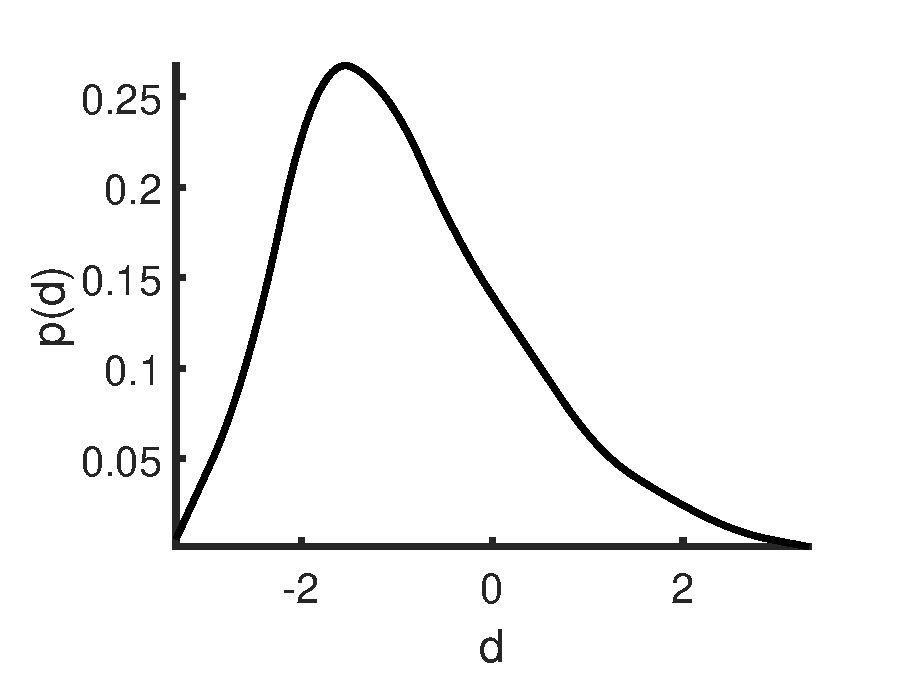
\includegraphics[width=0.2\textwidth]{fig_4a.eps}
}
\subfigure[Yahoo!user]{
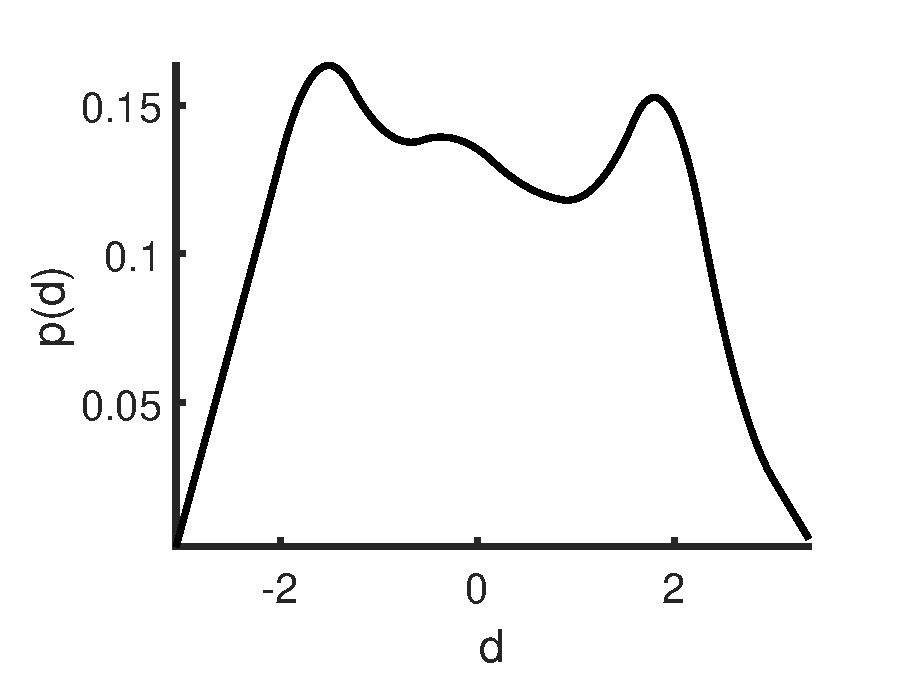
\includegraphics[width=0.2\textwidth]{fig_4b.eps}
}
\caption{The comparative probability distribution of rating divergence $d$ on different settings in Yahoo!}\label{fig:yahoo}
\end{figure}

 
 \subsection{Opinion Climate}
Opinion climate is a coined term to describe the mainstream opinion. For a thorough understanding of how the opinion climate develops and influences response patterns, we conduct the following studies on the Yahoo! data set.

In the theory, opinion climate is highly affected by the mass media. In recommender systems, opinion leaders play a similar role as mass media. For the cause of observing, we first select $10$ most active users $O$ (with largest number of ratings) as opinion leaders, and compute the average rating within opinion leaders $\hat{r_j}=[\Sigma_{i\in O}r_{i,j}][|O|]$. From Fig.~\ref{fig:leader}, we see that, the p.d.f of rating divergence to opinion leaders moves to the right in both settings. The difference between two settings is more obvious than divergence to average people. 

\begin{figure}[htbp]
\centering
\centering
\subfigure[Yahoo!random]{
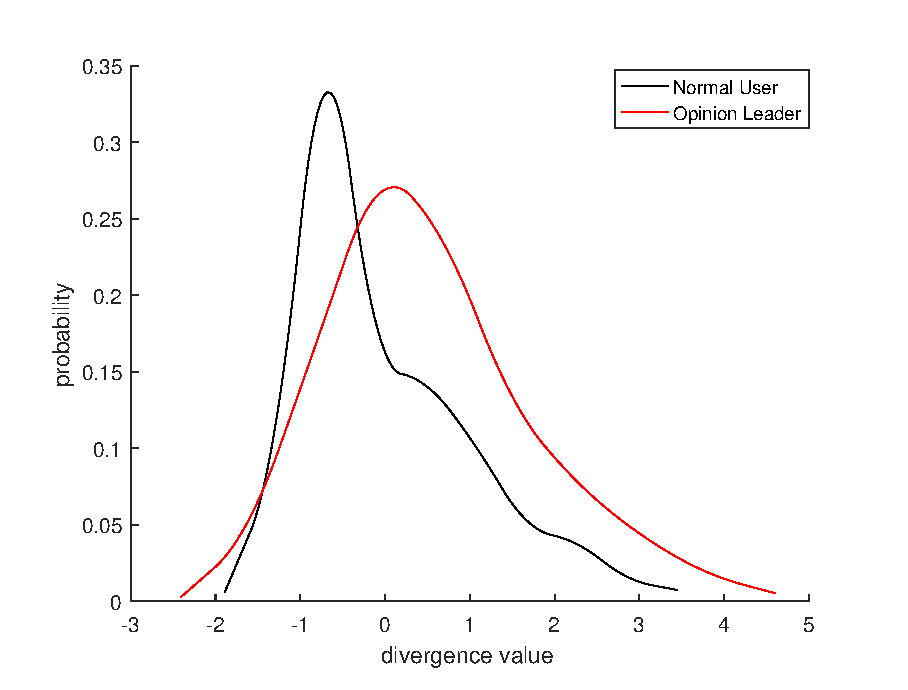
\includegraphics[width=0.2\textwidth]{fig5_random.eps}}
\subfigure[Yahoo!user]{
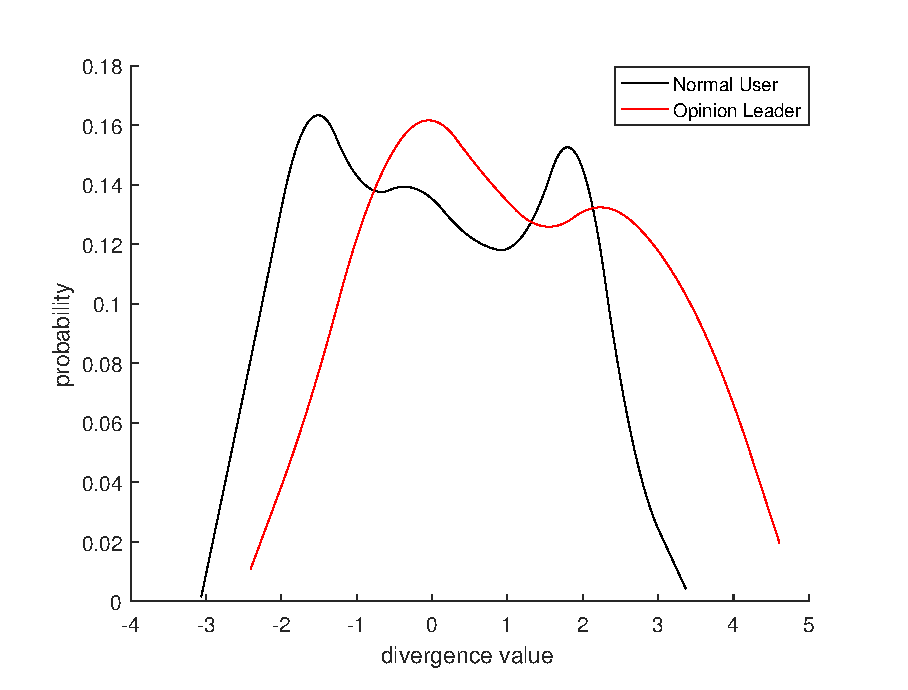
\includegraphics[width=0.2\textwidth]{fig5_user.eps}}
\caption{The comparative distribution of rating divergence $d$ to opinion leaders on different settings in Yahoo!}\label{fig:leader}
\end{figure}

Based on the above observation, we bootstrap $10$ opinion leaders from top $100$ active users. We use the \textbf{K}olmogorov-\textbf{S}mirnov (K-S) test to test if the rating divergence to opinion leaders is larger than that to all users. The null hypothesis that the samples are drawn from the same distribution. We obtain zero p values in $1000$ bootstrap runs. 

Past findings on characteristics of opinion leaders usually suggest that opinion leaders have large influence on others. We compute the  average rating divergence per user $I_i=[\Sigma_{j,t} d(r_{i,j,t})]/|\{r_{i,j,t}\}|$ to approach the strength of influence. Smallest $d_i$ indicates the user $i$ has strongest influence on the public opinion.  We bootstrap 10 users from $100$ users with the smallest $d_i$ for 1000 times. We conduct K-S test and again obtain zero p values in all runs. It shows that opinion leaders magnify users' willingness to remain silence when they hold negative feedback and speak out positive opinions.

On the Internet, with the infinite flow of information, users tend to have a limited vision of how others think and behave. They might focus on the opinions alike theirs, and thus perceive a so-called ``looking-glass perceptron'' of opinion climate. To study whether the opinion climate is dependent on user communities, we first represent each user as a rating vector on the item universe, and proceed to form a cluster $c$ for users by selecting the KNN ($K=50$) users with similar tastes.  We then compute the average of community ratings $\hat{r_{j,c}}=[\Sigma_{i\in c}r_{i,j}]/|c|$ for community $c$. For each user $u_i$ in community $c$, the rating divergence is   $d(r_{i,j})=r_{i,j}-\hat{r_{j,c}}$.

\begin{figure}[htbp]
\centering
\centering
\subfigure[Yahoo!random]{
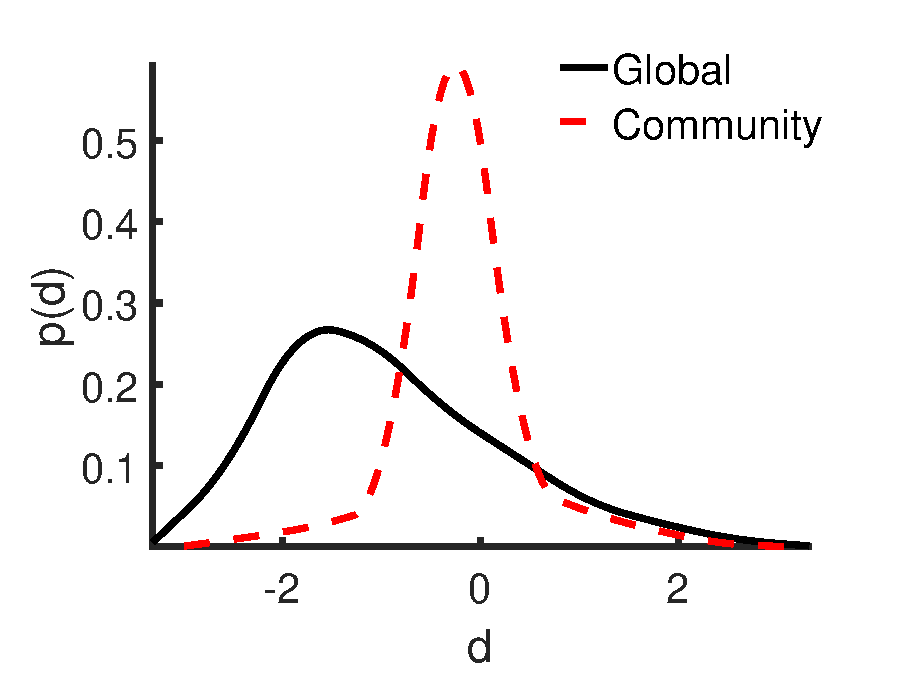
\includegraphics[width=0.2\textwidth]{fig_6a.eps}\label{fig:communityrandom}
}
\subfigure[Yahoo!user]{
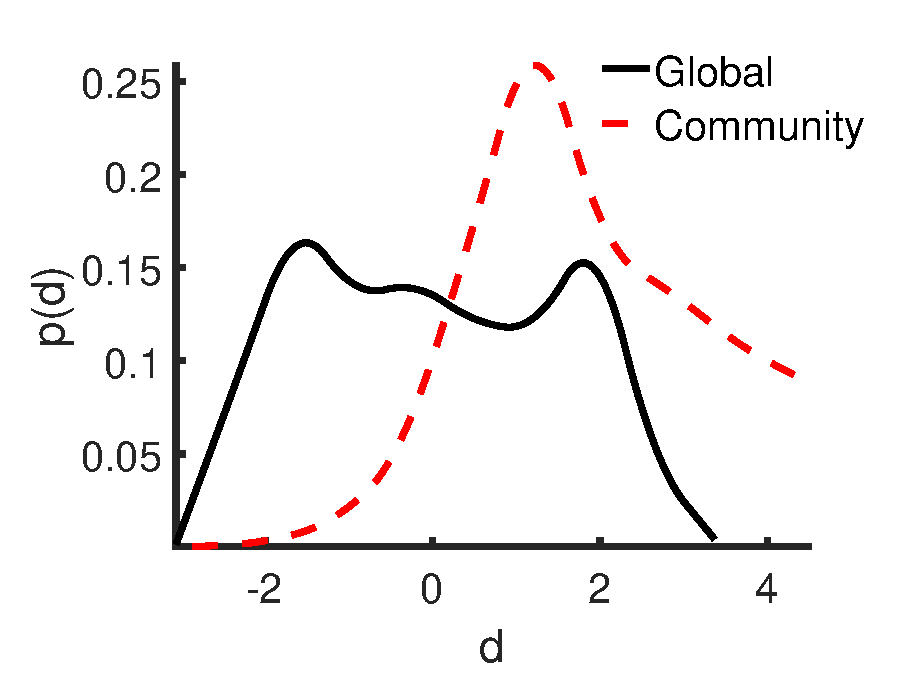
\includegraphics[width=0.2\textwidth]{fig_6b.eps}\label{fig:communityuser}
}
\caption{The comparative  distribution of community specific rating divergence $d$ on both settings in Yahoo!}\label{fig:community}
\end{figure}

As shown in Fig.~\ref{fig:community}, we have the following observations. (1) In the random setting, rating divergence to community specific majority rating follows a shallow normal distribution, which centers at around $0$.  (2) In the user selected setting, distribution of rating divergence to community specific majority rating is single peaked and asymmetric. The probability peak is at around $1.25$. The probability of negative feedback is much lower than rating divergence to global average rating. These observations strongly indicate that users perceive community specific opinion climate from his/her alike people.

\subsection{Hardcore Users}

In the theory, hardcore group is a bunch of people who are brave and willing to express different opinions. For simplicity, we ignore the possibility that users use pseudonyms. We assume that each user is unique and represents one person in reality. We define a ``hardcore'' score for each user:

\begin{equation}
h=\frac{n^h_i}{n_i},
\end{equation}

\noindent where $n_i$ is the number of ratings a user $i$ gives to all items, $n^h_i$ is the number of high divergent ratings of user $i$. In Eachmovie, high divergent ratings are $\{|r_{i,j}-\hat{r_{j}}|\geq 0.3\}$. In Movielens, CoAn and Yahoo!users, $\{|r_{i,j}-\hat{r_{j}}|\geq 1.5\}$. In Yahoo!random $\{|r_{i,j}-\hat{r_{j}}|\geq 1.0\}$ as the random data set consists less ratings. 

We first detect hardcore users in both yahoo data sets, and compare the hardcore users in two subsets. We report the overlap percentage $p_h=\frac{|G_{h}^{random}\bigcap G_{h}^{user}|}{|G_{h}^{random}\bigcup G_{h}^{user}|}$ in Tab.~\ref{tab:overlap}, where $G_{h}^{random},G_{h}^{user}$ are the set of hardcore users with hardcore score $h$ in the random subset and the user selected subset respectfully. We also provide the overlap percentage in theory given that users are uniformly sampled by the probability distribution of hardcore shown in Tab.~\ref{tab:hardcore}. We then conduct Mann-Whitney U test. The null hypothesis is that the distributions of actual and theoretical overlap are equal. We find that, despite of the threshold of hardcore score, the overlap percentage of hardcore users is always significantly larger than the theoretical overlap, However, the Mann-Whitney U test suggests that the overlap percentages under non-hardcore situations can not reject the null hypothesis (not shown in Tab.~\ref{tab:overlap}). Our findings suggest that, hardcore is a consistent personality of users, users do not randomly decide to act hardcore. 


\begin{table}[htbp]
\centering
\small
\caption{Percentage of hardcore group overlap. $*$ indicates the actual overlap is significantly larger than theoretical overlap with $p\leq 0.05$ based on Mann-Whitney U test.}\label{tab:overlap}
\centering
\begin{tabular}{|c|c|c|c|c|}
\hline
 Threshold & $h\geq 0.5$ & $h\geq 0.6$ & $h \geq 0.7$ & $h\geq 0.8$ \\\hline\hline
Actual Overlap& 0.1638* &	0.1174* &	0.0908* & 0.0719* \\\hline
Theoretical Overlap & 0.1169 &  0.0658 &  0.0341 & 0.0156\\
\hline
\end{tabular}
\end{table}

It is natural to relate hardcore with attitude certainty, while attitude certainty is represented by an extreme rating value. We then set $h\geq 0.5$ to detect hardcore users, and plot the ratio of extreme ratings versus non-extreme ratings for hardcore and non-hardcore users in all data sets. Extreme ratings are $1,5$ ratings in Movielens, CoAn and Yahoo! and $0,1$ ratings in Eachmovie. We can see from Fig.~\ref{fig:hardcore} that in common RS datasets, hardcore users have a higher median ratio of extreme ratings, and the tail is much longer. We also notice that when users are forced to express (the Yahoo!random set), the tendency is enhanced, the majority of hardcore users (from highest to lowest datum of the box) have a higher ratio of extreme ratings and the tail is shorter.  This observation is again a supplementary evidence of the clear pattern that hardcore users are stubborn and are more likely to give extreme ratings.

\begin{figure*}[htbp]
\centering
\noindent
\subfigure[Eachmovie]{
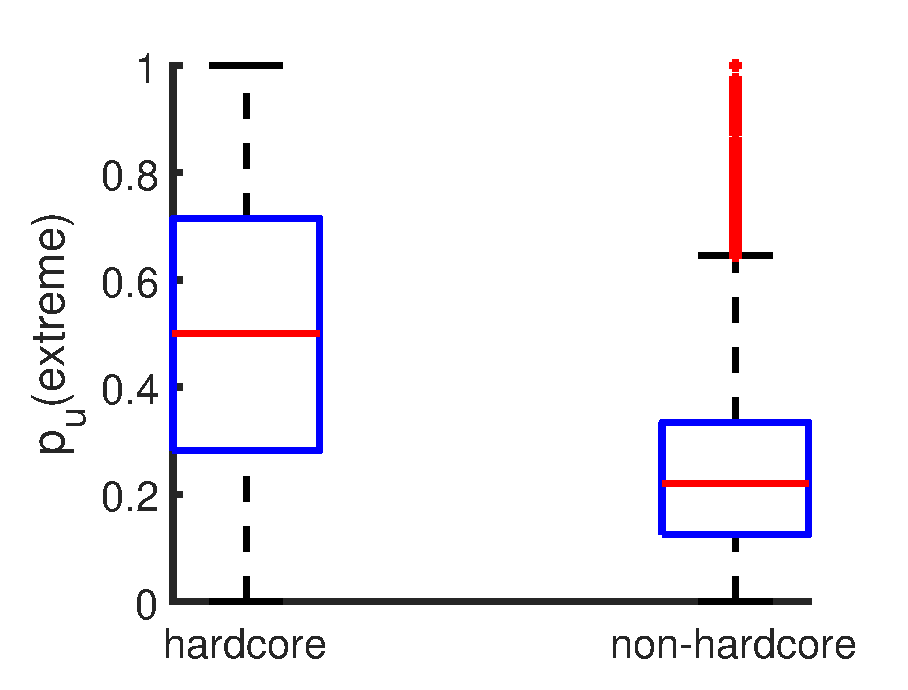
\includegraphics[width=0.18\textwidth]{fig_7a.eps}
}
\hspace{-0.5cm}
\subfigure[Movielens]{
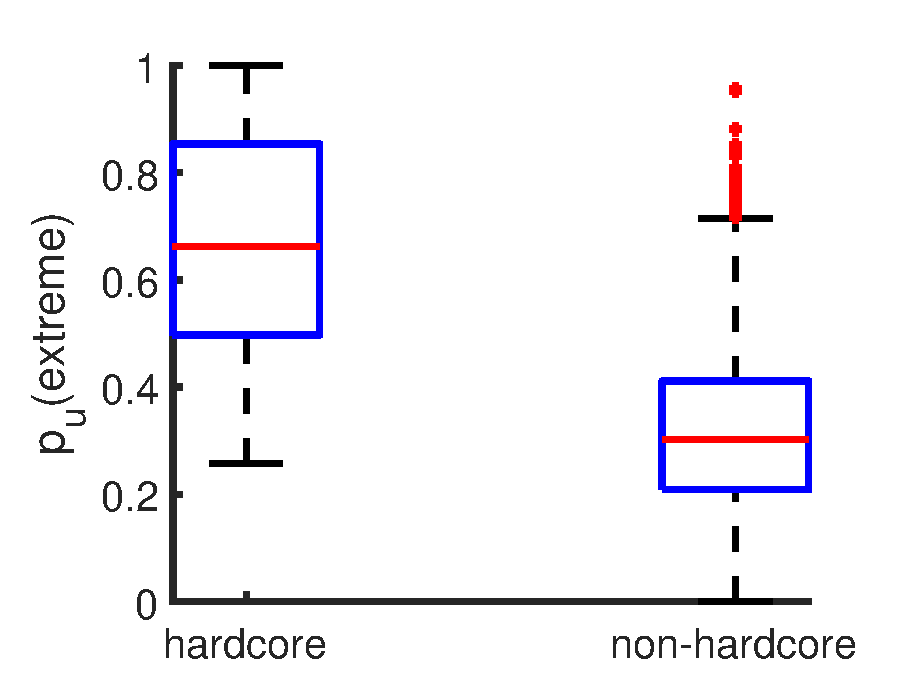
\includegraphics[width=0.18\textwidth]{fig_7b.eps}
}
\hspace{-0.5cm}
\subfigure[CoAn]{
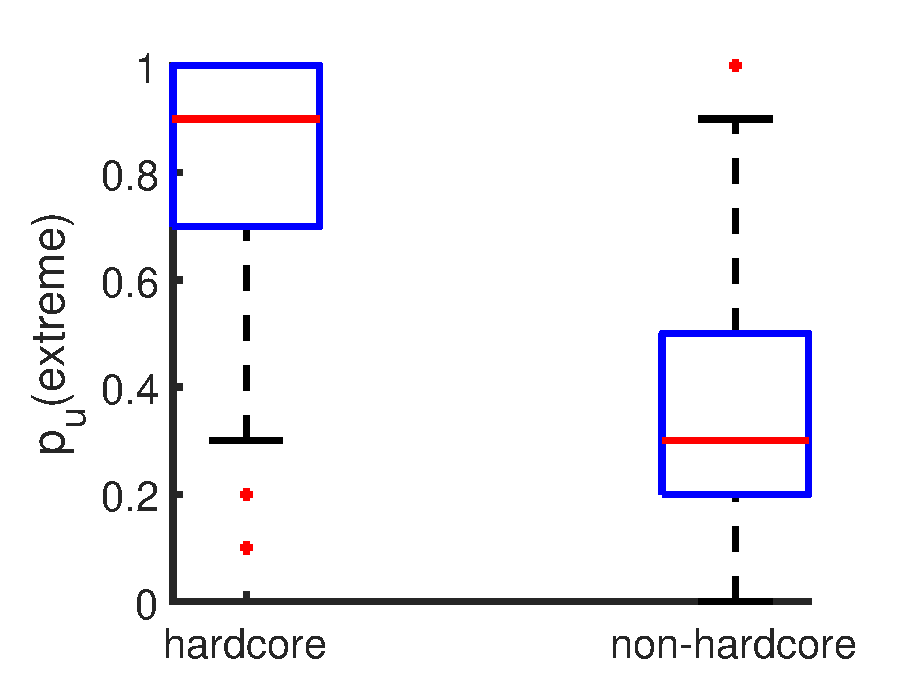
\includegraphics[width=0.18\textwidth]{fig_7c.eps}
}
\hspace{-0.5cm}
\subfigure[Yahoo!random]{
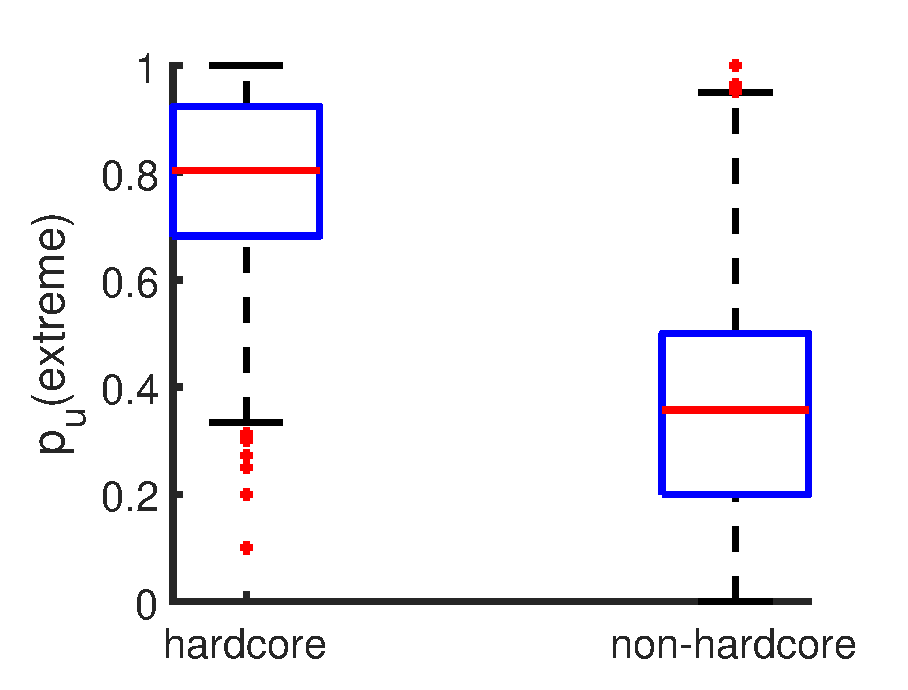
\includegraphics[width=0.18\textwidth]{fig_7d.eps}
}
\hspace{-0.5cm}
\subfigure[Yahoo!user]{
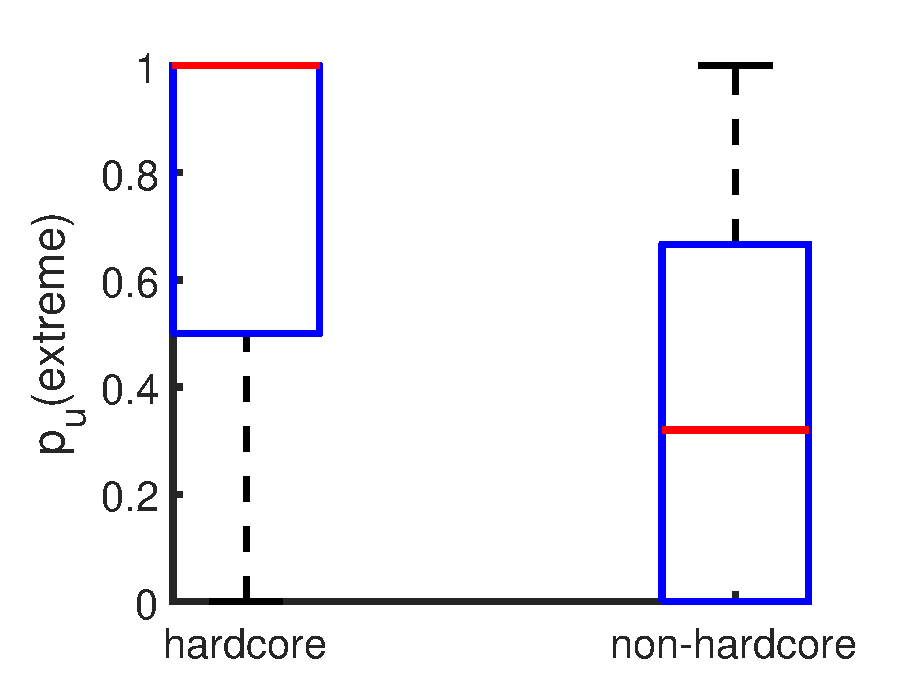
\includegraphics[width=0.18\textwidth]{fig_7e.eps}
}
\caption{Ratio of extreme ratings $p_u(extreme)$ for hardcore and normal users in Yahoo! datasets}
\label{fig:hardcore}
\end{figure*}

\subsection{Hardcore and Items}
Finally we study whether the strategies of holding back are dependent on the items. We first study whether the response is directly related to the popularity of items in Yahoo! datasets. We order the items in the Yahoo! data sets, according to the number of ratings assigned to them. Fig.~\ref{fig:popularity} reveals the distribution of rating divergence versus the order position of popularity. We can see that, in the random subset, the scales of rating divergence are almost the same for popular and unpopular items. In the user selected subset, the scale of rating divergence narrows as we choose less popular items. It shows that users adopt different strategies for popular items and unpopular items. When users are  not restricted,  they tend to give extreme ratings for popular items.

\begin{figure}[htbp]
\centering
\centering
\subfigure[Yahoo!random]{
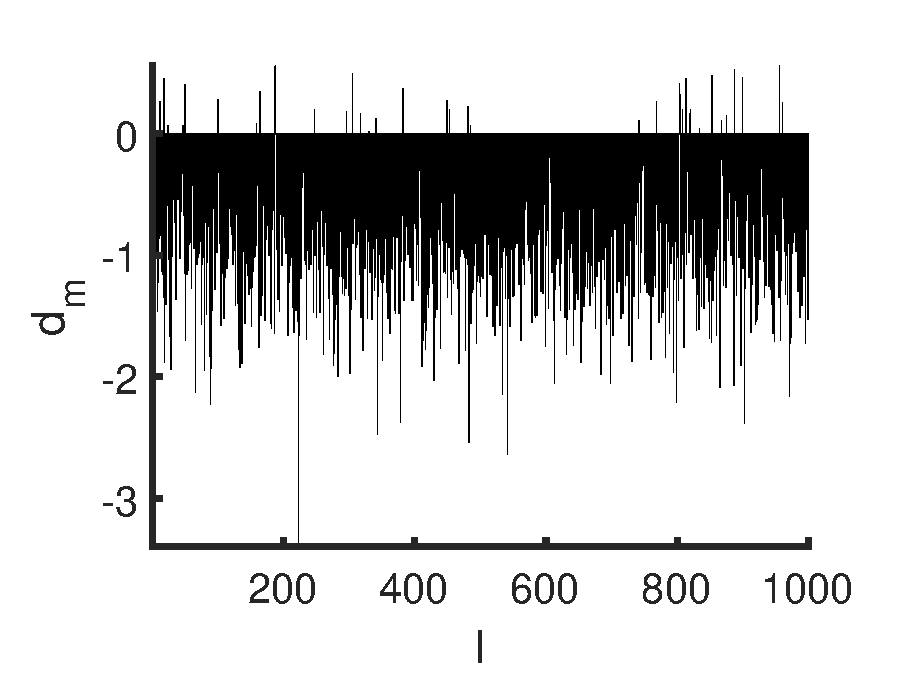
\includegraphics[width=0.2\textwidth]{fig_9a.eps}
}
\subfigure[Yahoo!user]{
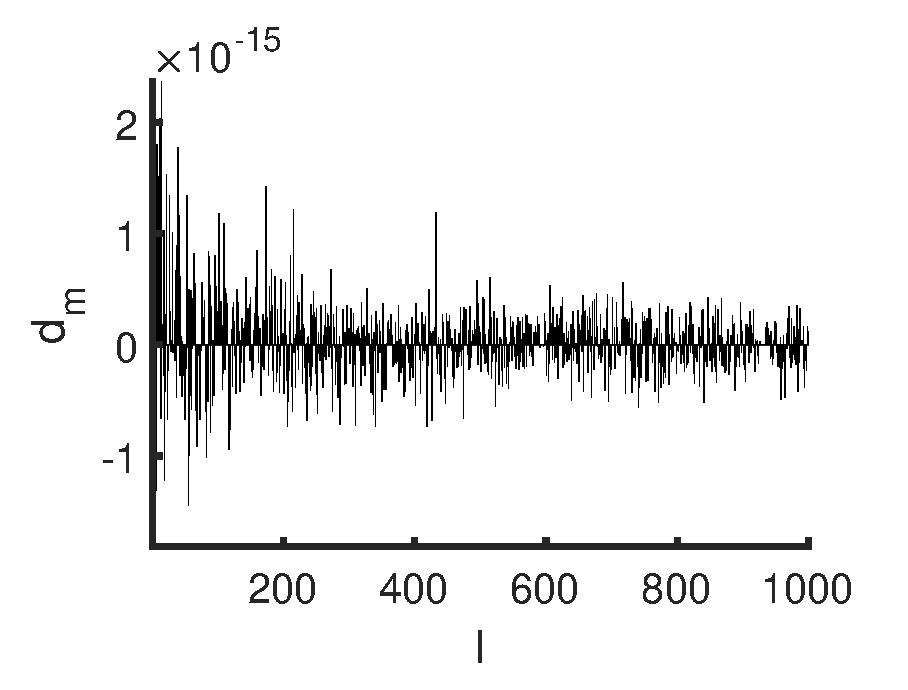
\includegraphics[width=0.2\textwidth]{fig_9b.eps}
}
\caption{The distribution of rating divergence $d_m$ upon item popularity index $l$}
\label{fig:popularity}
\end{figure}

We then test the above assumption on common RS datasets. At pre-processing, we filter items with too few ratings (number of ratings $\leq 50$). For each item, we compute the ratio of positive feedback in minority opinions $pos_r=|\{r_{i,jt}|d(r_{i,j,t})>a\}|/|\{r_{i,j,t}\}|$, and vice versa, the ratio of negative feedback $neg_r=|\{r_{i,jt}|d(r_{i,j,t})<-a\}|/|\{r_{i,j,t}\}|$, where $a=1$ in Movielens and CoAn, $a=0.2$ in Eachmovie. We then partition items to two groups, one group consists of items with much more positive feedbacks $pos_r-neg_r>0.1$, the other group consists of items with much more negative feedbacks $pos_r-neg_r<-0.1$ We then compare the popularity (number of ratings received) for each item in the two groups. We test by Mann-Whitney U (MWW) test if items with much more positive feedbacks receive significantly less ratings than items with much more negative feedbacks. As shown in Tab.~\ref{tab:popularity}, in all common RS datasets the popularity of the ``positive'' group is less than that of the ``negative'' group at significance level $5\%$. This again verifies that popular items receive more critics. 

\begin{table}[htp]
\caption{MWW test significance level of positive items being less popular than negative items on different datasets}
\begin{center}
\small
\begin{tabular}{|c|c|c|c|}
\hline
Dataset & Movielens & Eachmovie & CoAn \\\hline
\hline
p value & 0.0447 & 0.0435 & 0.0187 \\\hline 
\end{tabular}
\end{center}
\label{tab:popularity}
\end{table}

It is mentioned in the theory\cite{Neolle-Neumann1993spiral} that hardcore is related to personal interest or importance. To testify this assumption, we select the most rated tag and least rated tag (in number of ratings) for each user, and compute the hardcore score, where $n_i$ is the number of ratings a user $i$ gives to all items associated with the tag.  As shown in Fig.~\ref{fig:personalinterest}, in both data sets, users are more willing to express different opinions (with a higher hardcore score) for least interesting items.

\begin{figure*}[htbp]
\centering
\centering
\subfigure[Movielens]{
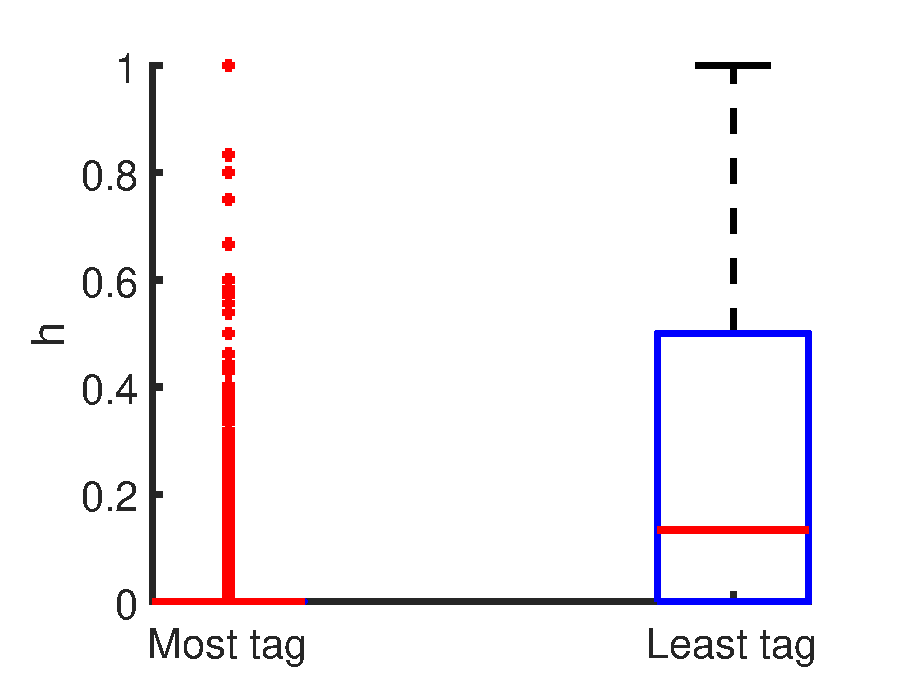
\includegraphics[width=0.2\textwidth]{fig_10a.eps}
}
\subfigure[Eachmovie]{
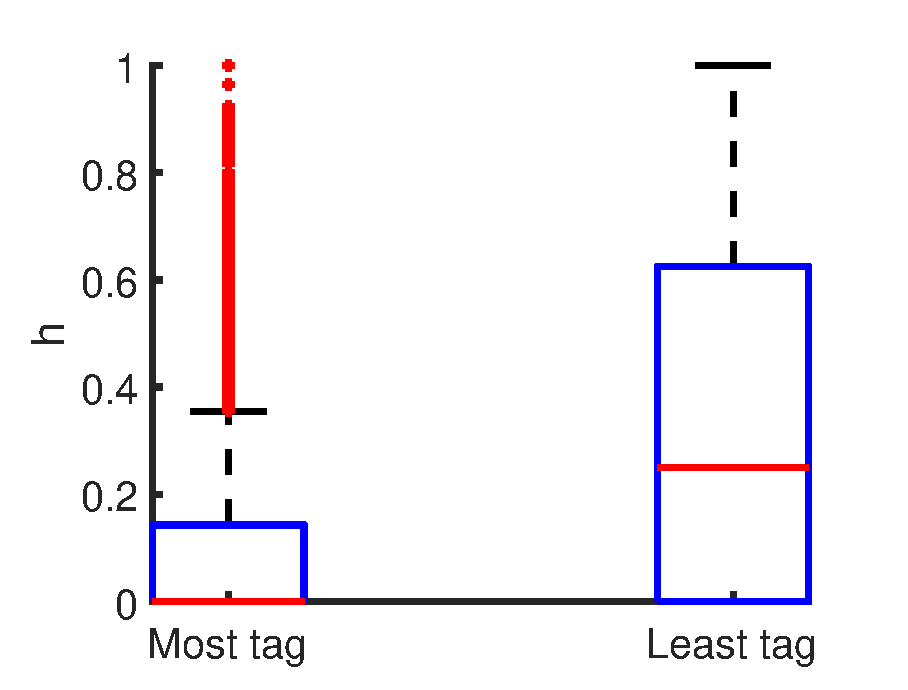
\includegraphics[width=0.2\textwidth]{fig_10b.eps}
}
\subfigure[CoAn]{
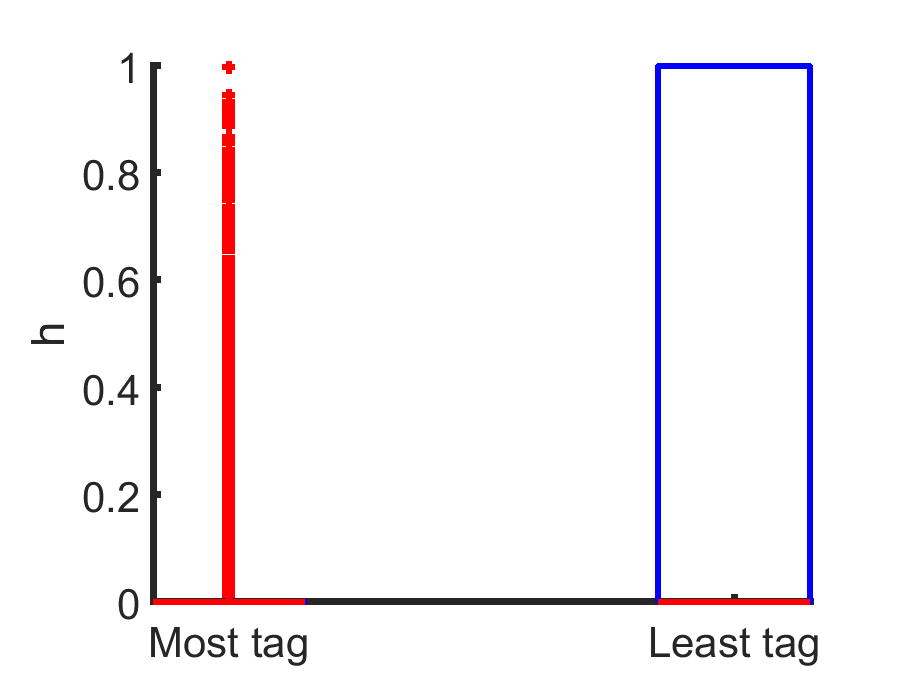
\includegraphics[width=0.2\textwidth]{fig_10c.eps}
}
\caption{The distribution of hardcore scores $h$ upon personal interest}
\label{fig:personalinterest}
\end{figure*}

Is hardcore related to moral basis? We define two moral situations in Recommender Systems, one is to praise a (wrongly) criticized item, the other is to criticize an (improperly) appreciated item. Following the definition of hardcore score, we compute how people react in giving positive feedback ($r_{i,j}>\hat{r}+\frac{\max{r}-\min{r}}{p}$, $p=5$ for Movielens, Eachmovie, CoAn and Yahoo!users, $p=10$ for Yahoo!random as this data set is much smaller) to items with average negative feedback ($\hat{r}< 3/5 (\max{r}-\min{r})$) and giving negative feedback ($r_{i,j}<\hat{r}-\frac{\max{r}-\min{r}}{n}$, $n=5$ for Movielens, Eachmovie and Yahoo!users, $n=10$ for Yahoo!random) to items with average positive feedback ($\hat{r}>3/5 (\max{r}-\min{r})$) . As shown in Fig.~\ref{fig:moralbasis}, in most cases people feel more obligated to save a criticized item than to underrate a highly appreciated item. The only exception is CoAn. Users in CoAn seem to be more critical than users in other platforms.

\begin{figure*}[htbp]
\centering
\noindent
\subfigure[Eachmovie]{
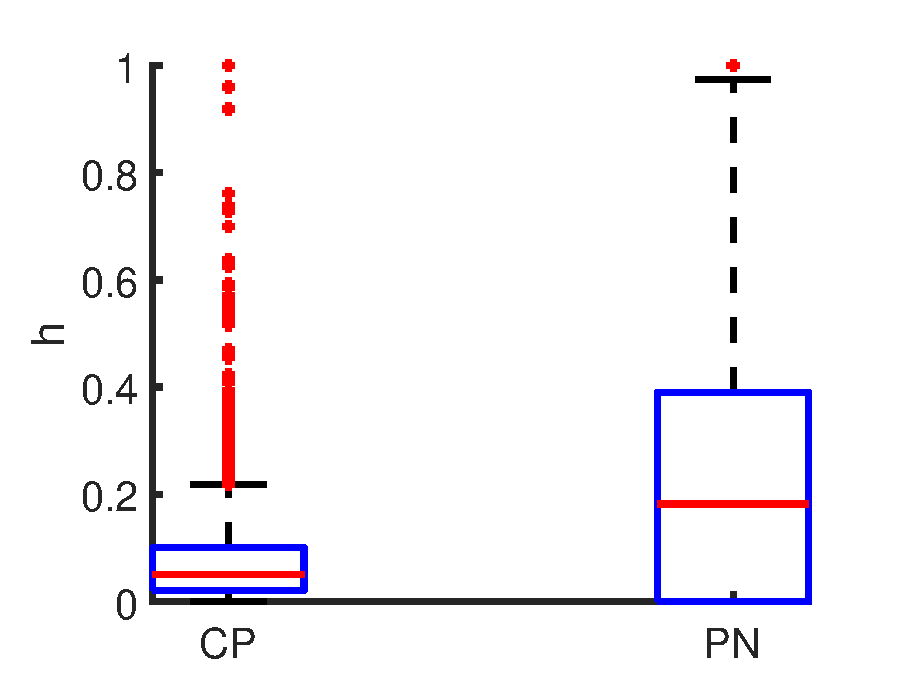
\includegraphics[width=0.18\textwidth]{fig_11a.eps}
}
\hspace{-0.5cm}
\subfigure[Movielens]{
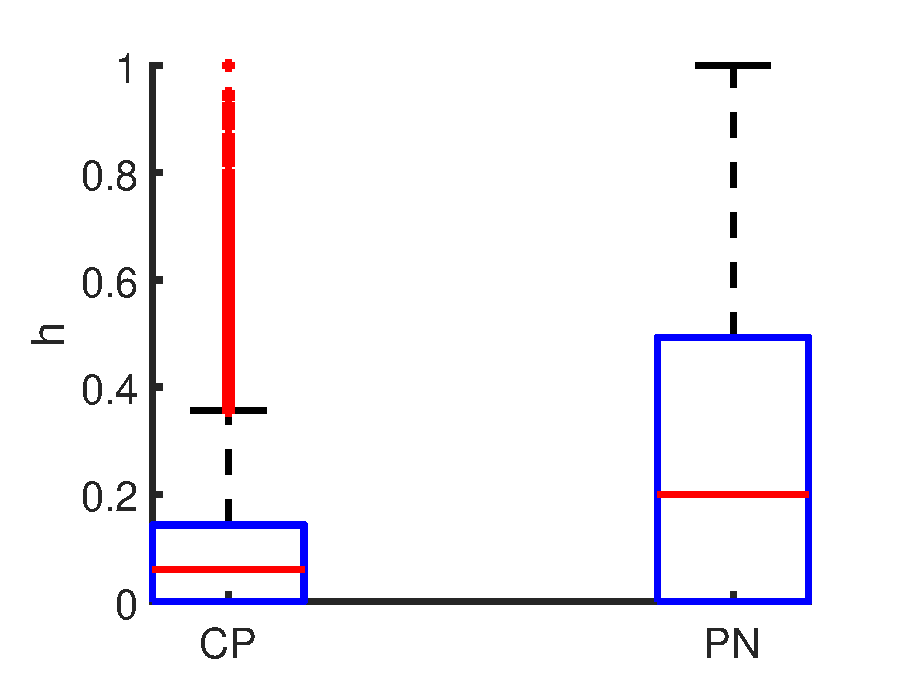
\includegraphics[width=0.18\textwidth]{fig_11b.eps}
}
\hspace{-0.5cm}
\subfigure[CoAn]{
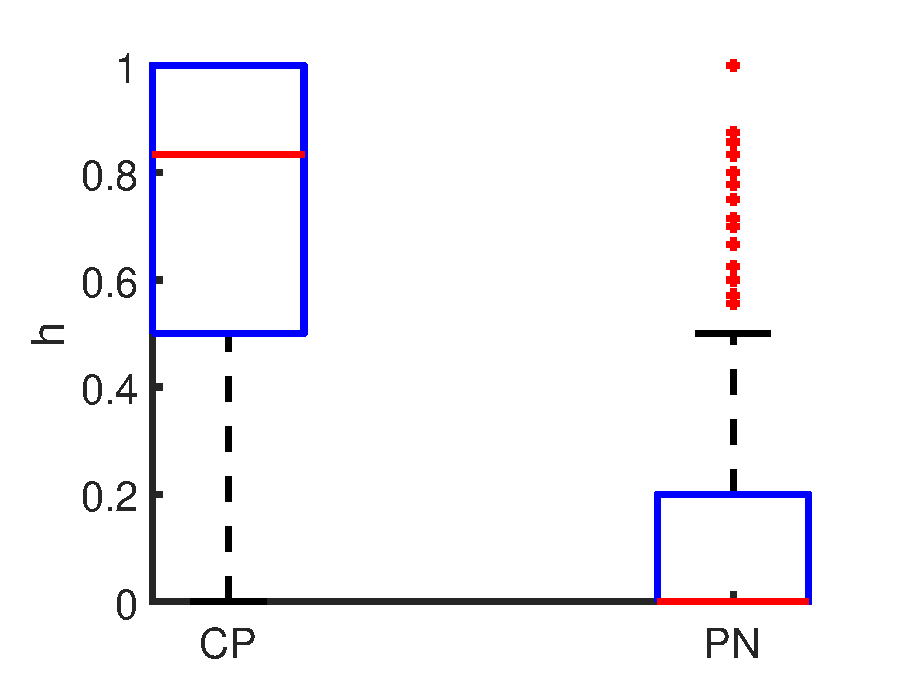
\includegraphics[width=0.18\textwidth]{fig_11c.eps}
}
\hspace{-0.5cm}
\subfigure[Yahoo!random]{
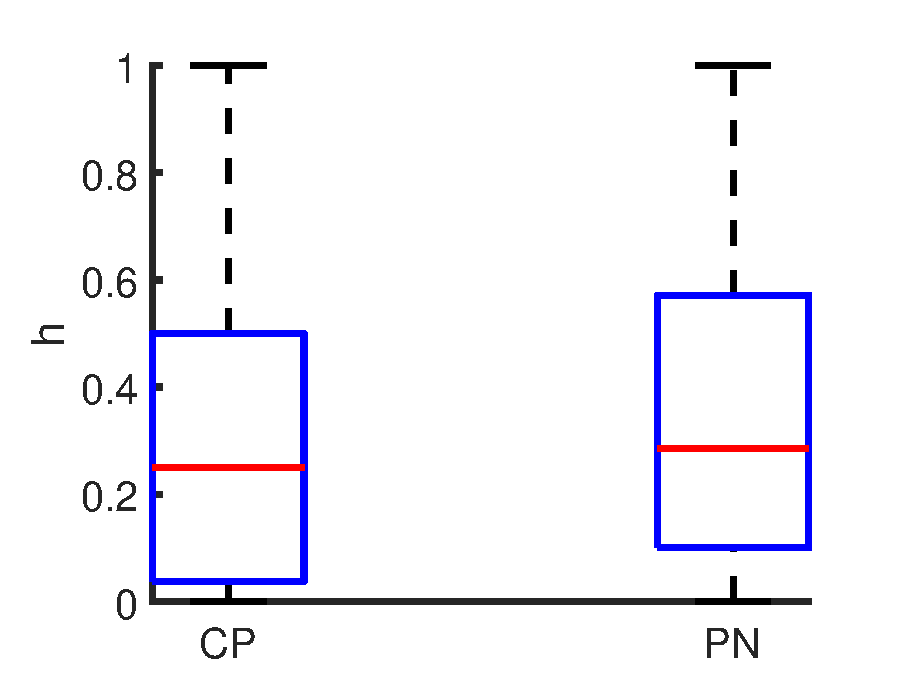
\includegraphics[width=0.18\textwidth]{fig_11d.eps}
}
\hspace{-0.5cm}
\subfigure[Yahoo!user]{
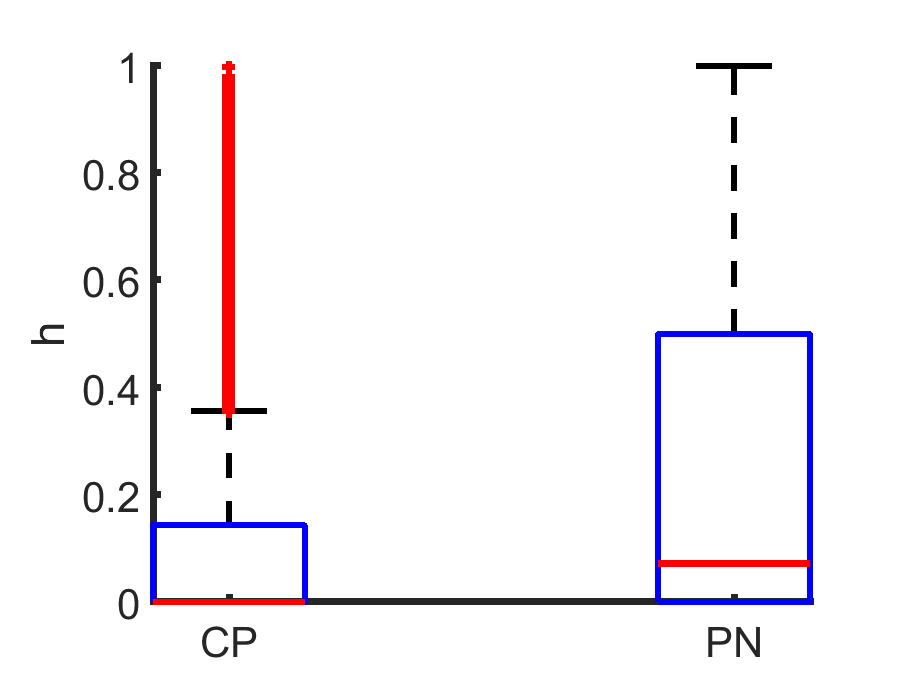
\includegraphics[width=0.18\textwidth]{fig_11e.eps}
}
\caption{Distributions of hardcore scores $h$ under two moral situations, CP (criticizing a positive item) and PN (praising a negative item)}
\label{fig:moralbasis}
\end{figure*}

We also conduct analysis to correlate hardcore personality to user experience and context of ratings. No evidence is found to imply significant correlation between the probability of a user being hardcore and the number of ratings he/she gives, in which day of a week and which time of a day the rating is given, and the previous items he/she rates. We omit the analysis here due to the limit of space.

\section{Model}\label{sec:model}

\begin{table}[htp]
\caption{Notations used in the models}
\begin{center}
\small
\begin{tabular}{|c|c|}
\hline 
Symbol & Semantics \\\hline
\hline
$U_i\in R^K$ & User preference \\\hline
$V_j \in R^K$ & Item feature \\\hline
$BU_i,BV_j\in R$ & User or item bias \\\hline
$R_{i,j}\in (0,1)$ & Rating \\\hline
$X_{i,j} \in \{0,1\}$ & Response \\\hline
$E_j\in (0,1)$ & Empirical majority opinion \\\hline
$OR_j\in (0,1)$ & Empirical leader's opinion \\\hline
$AU_i,AV_j\in R^K$ & User or item activity \\\hline
$VP_{i,j}\in R$ & User-item specific popularity \\\hline
$\gamma_{i,c}\in \{0,1\}$ & User-community assignment\\\hline
$\alpha\in R^C, \forall c, \alpha_{c}\in \{0,1\}, \Sigma_c\alpha_c=1$ & Global community distribution\\\hline
$\pi_i\in R^2, \forall z, \pi_{i,z}\in \{0,1\}, \Sigma_z \pi_{i,z}=1$ & User persona distribution\\\hline
$\tau_z\in R$ & Persona $z$'s hardcore coefficient \\\hline
\end{tabular}
\end{center}
\label{tab:notations}
\end{table}%



%basic MNAR model
As with most matrix factorization models, we assume there are $K$ hidden aspects. The user preference is denoted as a vector $U_i\in R^K$, and each item's coefficient to the aspects is denoted as a vector $V_j \in R^K$. The rating given by user $U_i$ to item $V_j$ is denoted by $R_{i,j}$. The ratings are semi-observed. Whether the rating $R_{i,j}$ is observed is denoted by a binary response variable $X_{i,j}$, where $X_{i,j}=1$ indicates the rating is observed and otherwise the rating is missing. Other notations are given in Tab.~\ref{tab:notations}. 

\begin{figure}[htbp]
\centering
\subfigure[Base $\&$ COL]{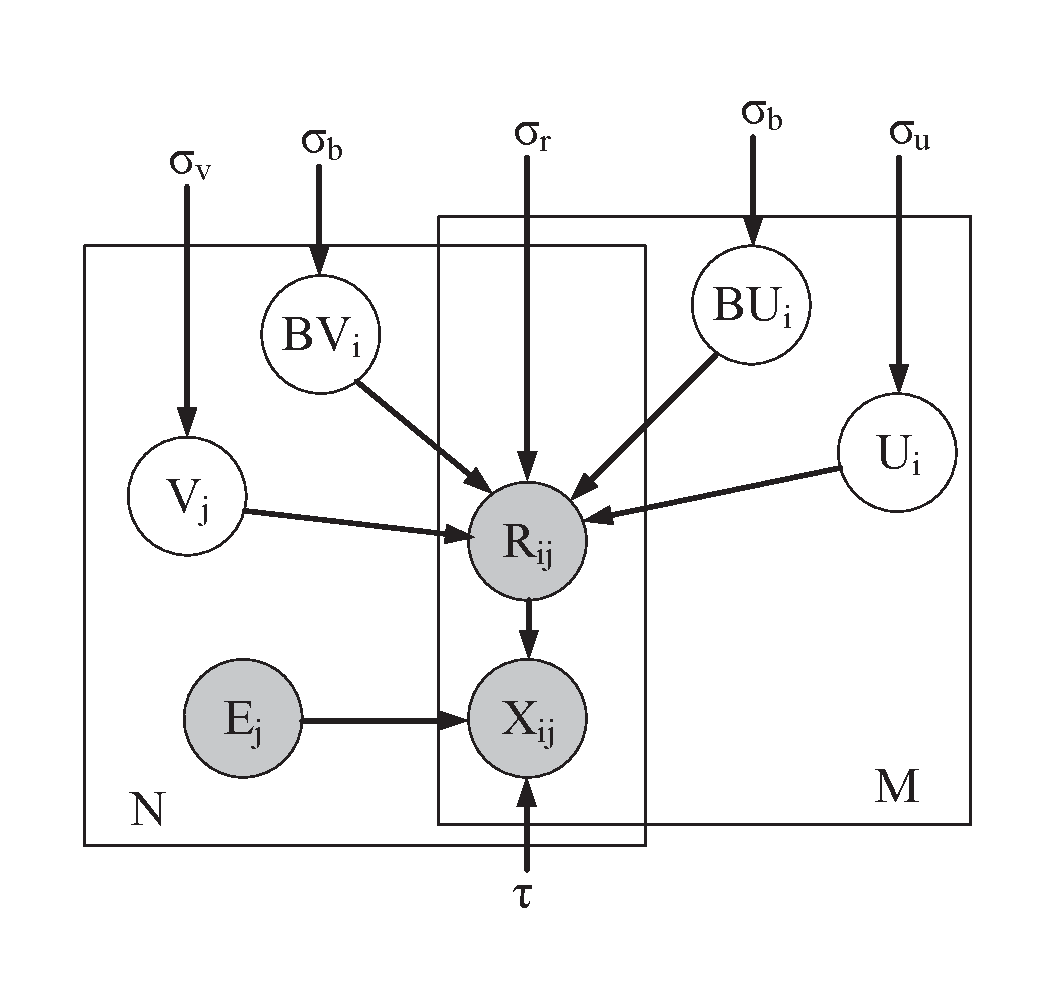
\includegraphics[width=0.2\textwidth]{fig12_Base.eps}\label{fig:basemodel}}
\vspace{-1em}
\hspace{-1em}
\subfigure[CPC]{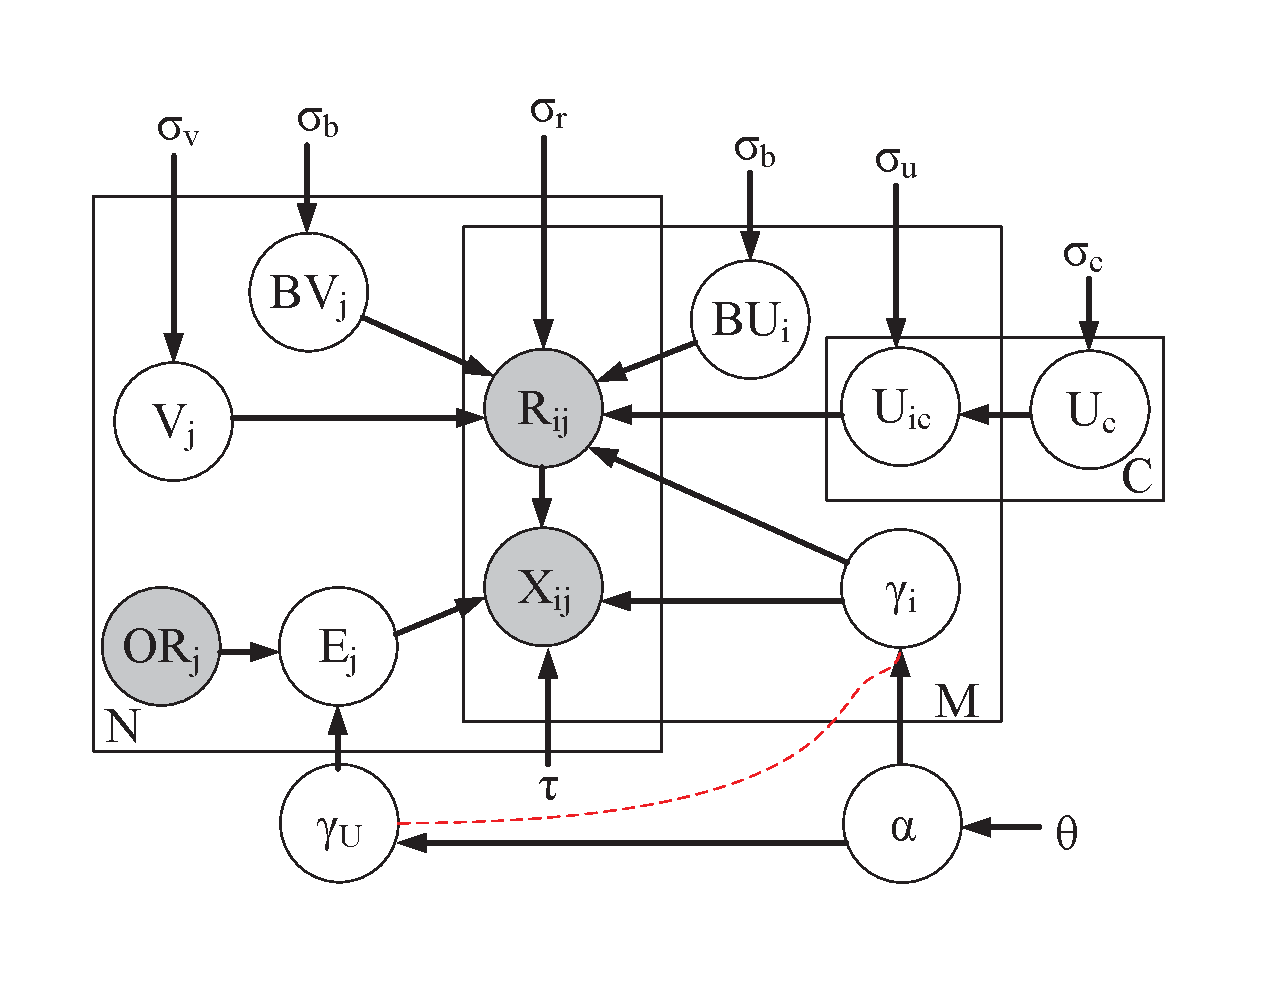
\includegraphics[width=0.25\textwidth]{fig12_CPC.eps}\label{fig:communitymodel}}
\vspace{-1em}
\subfigure[CPP]{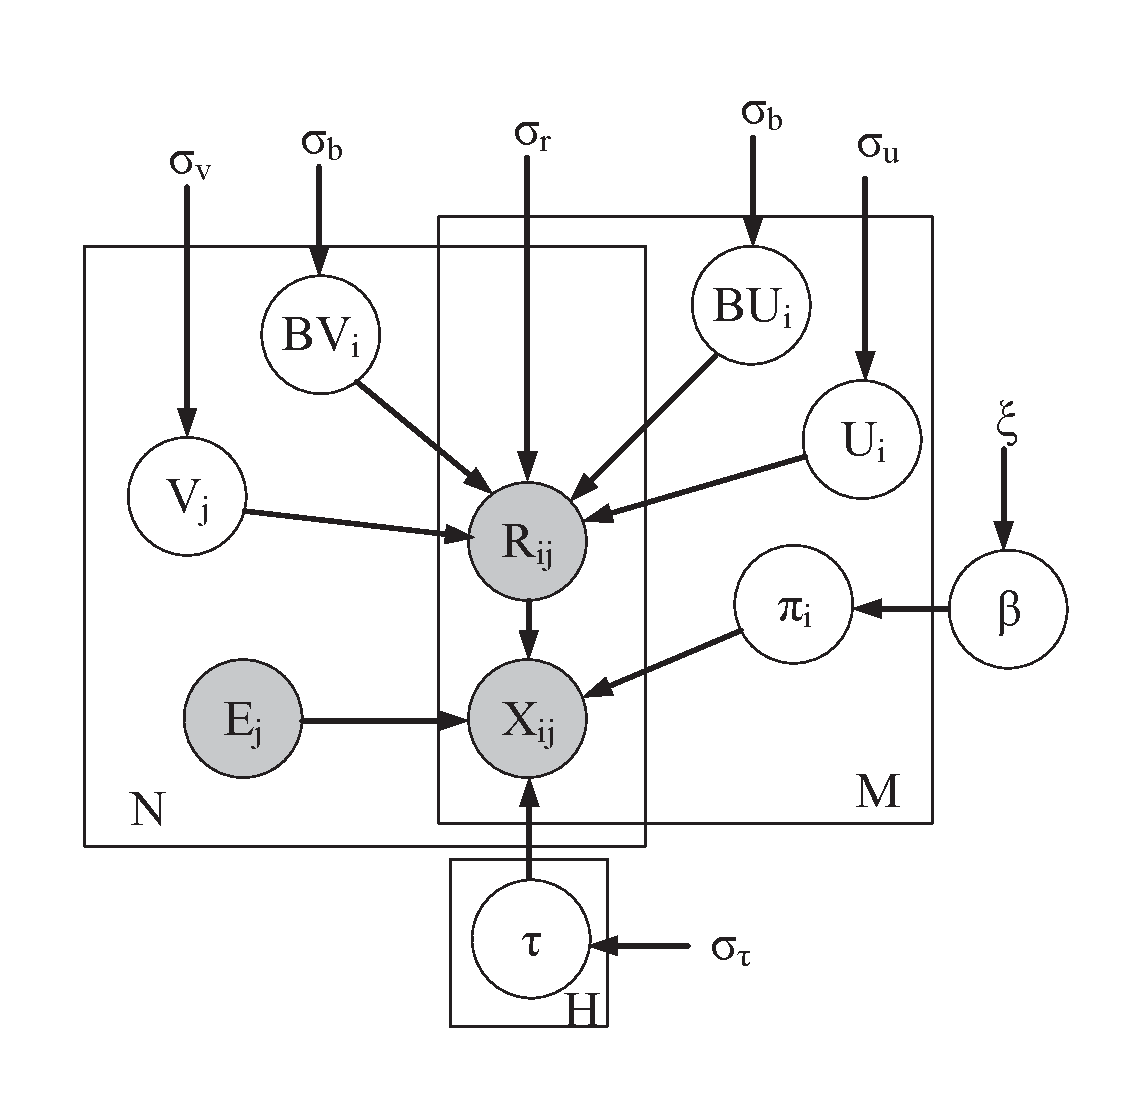
\includegraphics[width=0.23\textwidth]{fig12_CPP.eps}\label{fig:hardcoremodel}}
\hspace{-1em}
\subfigure[CPV]{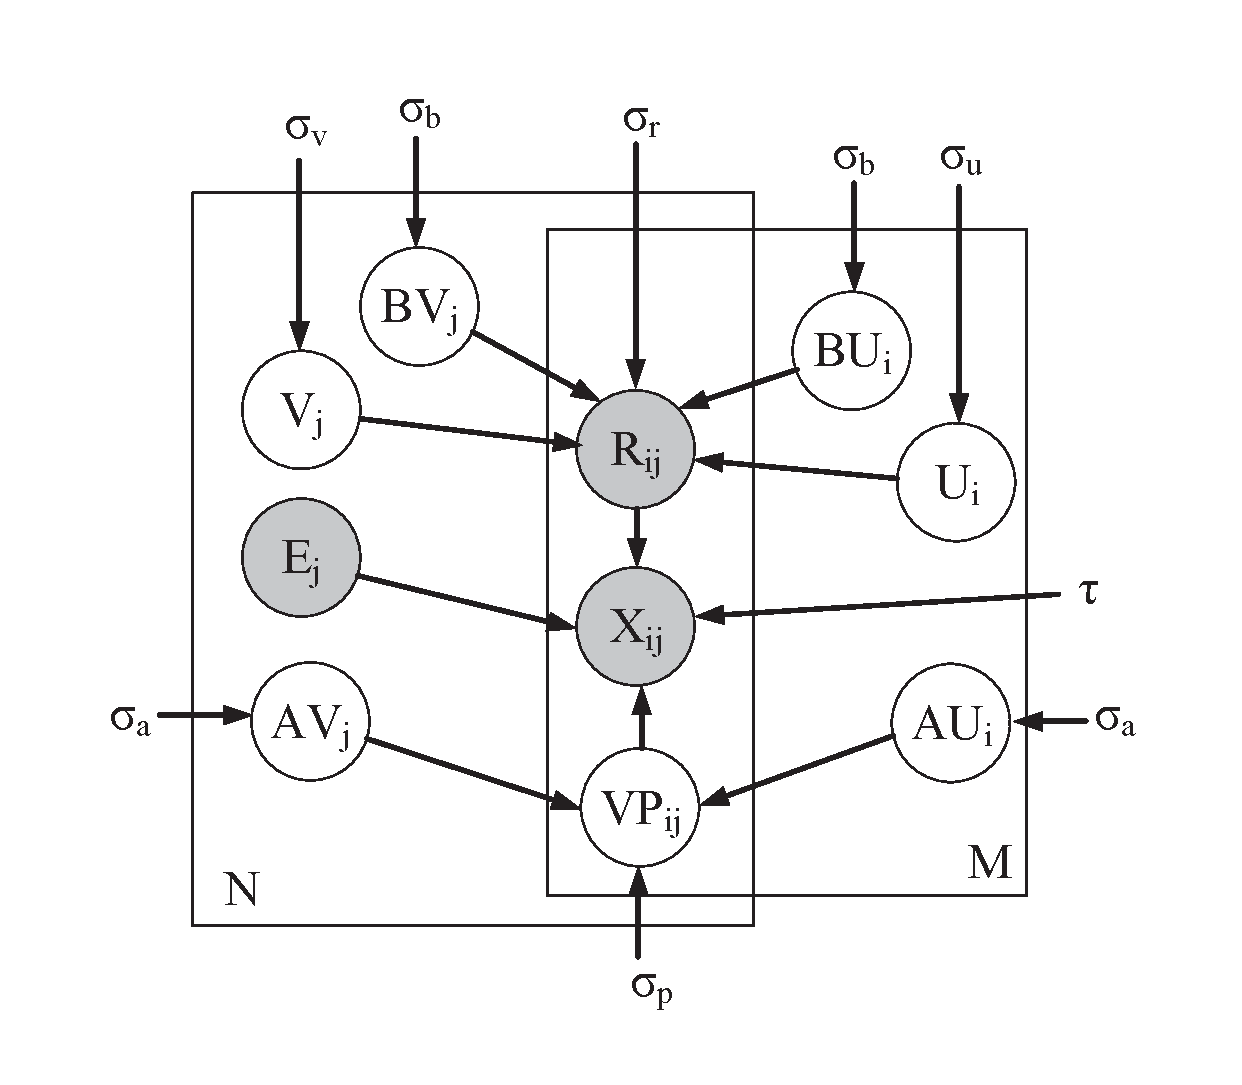
\includegraphics[width=0.23\textwidth]{fig12_CPV.eps}\label{fig:itemmodel}}
\caption{Graphic representation of models}\label{fig:model}
\end{figure}
\subsection{Basic Model}

Intuitively, a user will give a high rating if the item matches his/her preference. If his/her opinion is close to the opinion climate, he/she is more likely to reveal this rating. Furthermore, our  discovery in  empirical study shows that users feel more obligated to give positive feedback on negative items. Taking into account of the above three intuitions, our \textbf{Base} model assumes the following three generative stages.

\textit{The preprocessing stage:} For each user, generate the user preference from a Gaussian distribution with mean $0$.
\begin{equation}\label{equ:preferencebase}
U_i \sim \mathcal{N}(0,\sigma_u^2)
\end{equation}

Similarly, the user bias, item bias and item factors are also generated from Gaussian distributions. $BU_i, BV_j \sim \mathcal{N}(0,\sigma_b^2)$,  $V_j \sim \mathcal{N}(0,\sigma_v^2)$.

\textit{The rating generation stage:} The rating $R_{i,j}$ approaches to $U_iV_j+Bu_i + Bv_j $, with a  zero-mean Gaussian error. Hence in this stage, generate the rating: 

\begin{equation}\label{equ:rating}
R_{i,j} \sim \mathcal{N}(U_iV_j+BU_i+BV_j, \sigma_r^2)
\end{equation}

\textit{The response generation stage:} $p(X_{i,j}=1)$ increases with smaller rating divergence to opinion climate $R_{i,j}-E_j$. Generate the response value $X_{i,j}$ from Eq.\ref{equ:responsebase},

\begin{equation}\label{equ:responsebase}
 P(X_{i,j}=1|R_{i,j},E_j,\tau)=\frac{1}{1+\exp{(-\tau(R_{i,j}-E_j))}},
\end{equation}
where $\tau\in [0,1]$ is a hardcore strength parameter, $E_j$ is the opinion climate for the particular item $j$. In the Base model, we set the opinion climate to be the average of all observed ratings.
\begin{equation}\label{equ:ebase}
 E_j=\frac{\Sigma_jR_{i,j}X_{i,j}}{\Sigma_j X_{i,j}}
\end{equation}


%expert
We next present four variant models, each individually models one important discovery in our empirical study. With a simple modification in the Base model, we obtain the \textbf{Conditional on Opinion Leader} (COL) model. The graphical representation of Base and COL is illustrated in Fig.~\ref{fig:basemodel}. Instead of computing a global majority rating by Eq.\ref{equ:ebase}, the average is taken over some expert users $e$,

\begin{equation}\label{eexpert}
E_j = \frac{\Sigma_e R_{e,j}X_{e,j}}{\Sigma_e X_{e,j}},
\end{equation}
where the experts $e$ are extracted by expert identification algorithms. This allows the flexibility of utilizing side information sources, such as cascaded social networks, to recognize opinion leaders. 

\subsection{Model Conditional Probability on Community}
%community
Our empirical discovery suggests a user perceives a filtered opinion climate of people sharing similar preferences. In the \textbf{Conditional Probability on Community (CPC)} model, we introduce a random $C-$dimensional vector $\gamma_i$ to represent the community assignment of each user,  $\gamma_{i,c}\in \{0,1\}, \Sigma_c \gamma_{i,c}=1$.  


Intuitively, users in the same community are alike to each other. We assume that the ``common'' preference in community $c$ is denoted by $U_c$. Thus as summarized in Fig.~\ref{fig:communitymodel}, the \textit{preprocessing stage} is as follows.

Generate $C$ communities. For each community, $U_c$ is generated from a zero-mean Gaussian distribution $U_c \sim \mathcal{N}(0,\sigma_u^2)$. Generate a global community distribution from Dirichlet distribution $\alpha\sim Dir(\theta), \Sigma_c \alpha_c=1, \forall \alpha_c>0$. For each user, first generate the community indicator $\gamma_i \sim Discrete(\alpha)$, then generate the user preference according to his/her community:

\begin{equation}\label{equ:preferencebase}
U_i \sim \Pi_c \mathcal{N}(U_c,\sigma_u^2)^{\gamma_{i,c}}.
\end{equation}

Suppose $OR_j$ represents the observed ratings, $OR_{i,j}=R_{i,j}X_{i,j}$, in the \textit{response generation stage}, we replace the opinion climate in Eq.\ref{equ:ebase} by a community specific opinion climate:  

\begin{equation}\label{equ:ecommunity}
 E_{c,j}=\frac{\Sigma_j\gamma_{i,c} OR_{i,j}}{\Sigma_i \gamma_{i,c} X_{i,j}}.
\end{equation}

\subsection{Model Conditional Probability on Persona}
%user personality
To model the split of users between hardcore and normal groups, the  \textbf{Conditional Probability on Persona (CPP)} model,  shown in Fig.~\ref{fig:hardcoremodel}, introduces a  persona variable,  denoted by $\pi \in \{0,1\}$. Intuitively, when a user is hardcore $\pi_{i,0}=1$, he/she is more likely to speak out regardless of the opinion climate. Thus the strength parameter $\tau$ is reasonably smaller.  Model Base,COL, CPC and CPV use a global $\tau$ for every user. In model CPP, $\tau$ is personalized for each persona.

In the \textit{preprocessing stage}, draw a persona distribution from a Beta distribution $\beta \sim \mathcal{Beta}(\xi), 0<\beta<1$. For each persona, Draw a hardcore coefficient $\tau_z \sim \mathcal{N}(1,\sigma_\tau), z\in \{0,1\}$. For each user, draw a persona from a Bernouli distribution $\pi_i \sim \mathcal{Bern} (\beta)$. 

The response probability is dependent on the user's persona $\pi_i$ and the hardcore strengths $\tau$ for each persona. In the \textit{response generation stage}, generate the response value $X_{i,j}$ from Eq.\ref{equ:responseCPP}:

\begin{equation}\label{equ:responseCPP}
 P(X_{i,j}=1|R_{i,j},E_j,\pi_i,\tau)=\Pi_z \frac{1}{{[1+\exp{(-\tau_z(R_{i,j}-E_j))}]}^{\pi_{i,z}}}.
\end{equation}

\subsection{Model Conditional Probability on Popularity Value}
%item popularity
Finally we give model \textbf{Conditional Probability on Popularity Value} (CPV) to associate the silence strategy to the nature of items. Our empirical findings reveal that users are less hardcore when it comes to his/her favorite items and niche items. Intuitively, in the generation of response, there is a hidden variable that interacts with both users and items. As shown in Fig.~\ref{fig:itemmodel}, in the \textit{preprocessing stage}, we introduce auxiliary variable $AU_i\in R^K$ to represent user attention on $K$ categories, $AV_j\in R^K$ to represent item's ``absence''. We have  $AU_i, AV_j \sim \mathcal{N}(0,\sigma_a^2)$.


In the \textit{rating generation stage}, we have $VP_{i,j}$ to represent item-user-specific popularity. in addition to Eq.~\ref{equ:rating}, let $VP_{i,j}$ to be sampled by:

\begin{equation}\label{equ:popularity}
VP_{i,j}\sim \mathcal{N}(AU_i AV_j,\sigma_p^2). 
\end{equation} 

Intuitively, if a user pays more attention to a category, and the item is absent from the best seller in the category, then it is less likely a different rating $r_{i,j}$ to be voiced.  Consequently, we modified the response probability to

\begin{equation}\label{equ:responseCPV}
P(x_{i,j}|r_{i,j},E_{j},\tau)=\frac{1}{1+\exp{(-\tau(r_{i,j}-E_{j}-VP_{i,j}))}}.
\end{equation}



\subsection{Inference}

The update equations in the four models share a similar form. For computational convenience, we first obtain $B_{i,j,c}$ and $p_{i,j,c}$ for each user, item and community at an iteration. Then we update $U_i$ and $V_j$ as follows.

\begin{shrinkeq}{-2ex}
\begin{equation}\label{equ:update}
\begin{split}
&p_{i,j,c}=U_{i,c}^{T}V_{j} + BU_{i} + BV_{j} \\
&B_{i,j,c}=(R_{i,j}-p_{i,j,c})^{[X_{i,j}=1]}(-\tau \mathcal{LS}(-\tau(p_{i,j,c}-E_{c,j})))^{[X_{i,j}=0]} \\
&U_{i,c}\leftarrow U_{i,c}+lr(\hat{\gamma}_{i,c}\sum\limits_{j=1}^{N}B_{i,j,c}V_j-(U_{i,c}-U_c)) \\
&V_j\leftarrow V_j+lr(\sum\limits_{c=1}^{C}\sum\limits_{i=1}^{M}\hat{\gamma}_{i,c}B_{i,j,c}U_{i,c}-V_j), 
\end{split}
\end{equation}
\end{shrinkeq}
where $\mathcal{LS}(x)=\frac{1}{1+\exp(-x)}$ is a logistic function, $lr$ is the learning rate. For model Base and COL, the c subscript is ignored (i.e. $p_{i,j,c}$ to $p_{i,j}$, $B_{i,j,c}$ to $B_{i,j}$), and set $\hat{\gamma}_{i,c}=1$. 

For the CPC and CPP models, we apply EM algorithm to infer the model parameters. In the E-step we need to compute $\omega_{i,j,*}$ for each user, item and community $c$ ($*=z$ for persona in CPP):

\begin{equation}
\omega_{i,j,*}=
\begin{cases}
P(X_{i,j}=1|R_{i,j},E_{j})P(R_{i,j}),& \text{$X_{i,j}=1$}\\\nonumber
1-P(X_{i,j}=1|R_{i,j},E_{j}),& \text{$X_{i,j}=0$}.
\end{cases}
\end{equation}

The hidden community $c$ is then inferred by

\begin{equation}\label{equ:updateCPC}
\begin{split}
&\hat{\gamma}_{i,c}\leftarrow\frac{\alpha_c\prod_{j=1}^{N}\omega_{i,j,c}}{\sum_{c=1}^{C}\alpha_c\prod_{j=1}^{N}\omega_{i,j,c}}. 
\end{split}
\end{equation}

For the CPP model, we update the following variables:
\begin{equation}
\begin{split}
&\hat{\pi}_{i,z}\leftarrow\frac{\beta_z\prod_{j=1}^{N}\omega_{i,j,z}}{\sum_{z=0}^{1}\beta_z\prod_{j=1}^{N}\omega_{i,j,z}} \\
&B_{i,j,z}=(R_{i,j}-p_{i,j})^{[X_{i,j}=1]}(-\tau_{i,z}\mathcal{LS}(-\tau_{i,z}(p_{i,j}-E_{j})))^{[X_{i,j}=0]} \\
&U_{i}\leftarrow U_{i}+lr(\sum\limits_{z=0}^{1}\hat{\pi}_{i,z}\sum\limits_{j=1}^{N}B_{i,j,z}V_j-U_{i}) \\
&V_j\leftarrow V_j+lr(\sum\limits_{z=0}^{1}\sum\limits_{i=1}^{M}\hat{\pi}_{i,z}B_{i,j,z}U_{i}-V_j).
\end{split}
\end{equation}

For  model CPV,  we ignore the c subscript, set $\hat{\gamma}_{i,c}=1$ and replace $E_{c,j}$ by $E_{c,j}=E_{j}+VP_{i,j}$, where $VP_{i,j}$ is updated by

\begin{equation}
\begin{split}
&D_{i,j}=\tau(\mathcal{LS}(-\tau(R_{i,j}-E_{j}))-1)^{[X_{i,j}=1]}(\mathcal{LS}(-\tau(p_{i,j}-E_{j})))^{[X_{i,j}=0]} \\
&AU_{i}\leftarrow AU_{i}+lr(\sum\limits_{j=1}^{N}D_{i,j}AV_j-AU_{i}) \\
&AV_{j}\leftarrow AV_{j}+lr(\sum\limits_{i=1}^{M}D_{i,j}AU_{i}-AV_j) \\
&VP_{i,j} \leftarrow AU_{i}^{T}AV_{j}.
\end{split}
\end{equation}

\section{Experiment}\label{sec:experiment}

The data sets used in this section include Yahoo!, MovieLen-1M, and Eachmovie mentioned above. In addition, we use the Mtweet benchmark with $106,337$ ratings by $3,972$ users on $2,043$ movies crawled from social network. In each data set, we remove users whose number of ratings is less than 10, and items which have less than 10 ratings. For each user, we randomly select 5 ratings to construct the test data sets. All ratings are converted to the range of $(1,5)$.


\subsection{Comparative Study}\label{sec:ndcg}

The major evaluation metric is $NDCG@L$, which is a standard measure for ranking systems.   NDCG@L is short for the normalized discounted cumulative gain for top $L$ results. 
\begin{equation}
NDCG@L=\sum\limits_{i=1}^{M}\frac{\sum_{l=1}^{L}(2^{r_{i}(p(l,i))}-1)/log(1+l)}{M\sum_{l=1}^{L}(2^{r_{i}(t(l,i))}-1)/log(1+l)},
\end{equation}
where $r_i$ is the relevance score for rank $i$, $p(l,i)$ is the index of the test items sorted in descending order by predicted ratings, $t(l,i)$ is the index of the test items sorted in descending order by true ratings.

The comparative $NDCG$ is conducted on Yahoo!random dataset. Evaluating $NDCG@L$ on a randomly missing data set, such as Yahoo!random, has been used as the primary criteria in many MNAR researches~\cite{Hernandez-Lobato2014Probabilistic,Marlin2009Collaborative}. Experiments on other non-randomly missing datasets could be misleading as the ground truth does not accurately reflect user preferences. Therefore, $NDCG$ on Yahoo!random dataset is the primary evaluation metric in this work. 

In all our models, we set the aspect numbers $K=5$, community numbers $C=2$, hyper-parameters  $\tau=1$ for models Base, COL, CPC and CPV.  $\xi=\theta=2$. All the variances are set to $\sigma_b=\sigma_a=\sigma_r=\sigma_u=\sigma_v=\sigma_\tau=1$. In COL, the top 10 users with most ratings on each item are selected as opinion leaders for this item. The learning rate is set to $lr=0.0001$ in Yahoo!, Mtweet and movieLen-1M, $lr=0.001$ in Eachmovie. Convergence is obtained when the change in mean log-likelihood $\Delta\bar{L}<0.0001$ or stopped at maximal $1500$ rounds.  

We compare our models to a wide range of available models, including conventional memory-based and model-based collaborative filtering recommenders, MNAR models, and ranking based models. The comparative models include (1)uKNN: the user based K-Nearest Neighbor collaborative filtering recommender; (2) MF: the standard matrix factorization model~\cite{Koren2009Matrix}; (3)PMF: the probabilistic matrix factorization model~\cite{salakhutdinov2008probabilistic}; (4)BPR: a classic ranking based model~\cite{Rendle2009BPR} (4)CPT-v and Logit-vd: the first MNAR models~\cite{Marlin2009Collaborative} with $K=10$; (5) MF-MNAR~\cite{Hernandez-Lobato2014Probabilistic}: the probabilistic MNAR model which masks the rating matrix by a response matrix, we set $K=20$; (6)RAPMF~\cite{Yang2015Boosting}: an MNAR model which incorporates users' response models into the probabilistic matrix factorization (parameter $K=5$). The parameters (including $K$ and variance $\sigma^2$) for the above models are tuned by cross validation.

As shown in Fig.~\ref{fig:modelNDCG} and Fig.~\ref{fig:compNDCG}, we can see that (1) The four variants of our model outperform all non ranking-based models in terms of NDCG at different lengths, which demonstrates the dominant advantages of adjusting a opinion climate in the MNAR models.  (2) CPC performs consistently best in all NDCGs. CPC outperforms the best state-of-the-art MNAR  models (MF-MNAR) for more than $10\%$ in all NDCGs. CPC is even better than ranking based models. For NDCG at less than top $5$ results, CPC boosts the performance for more than $5\%$ than the best of ranking based models (BPR). It proves the compactly of our approach. (3) COL, CPP and CPV are better than the base model, which verifies our empirical findings. (4) COL, CPP and CPV perform slightly worse than CPC. A possible explanation is that the user's perceives of opinion climate is mostly affected by the community. (5) BPR is the second best in all NDCGs. Because BPR directly optimizes the ranking of items, it is reasonable that it outperforms other rating optimization models.  


\begin{figure}[!htbp]
\centering
\subfigure[Our models]{
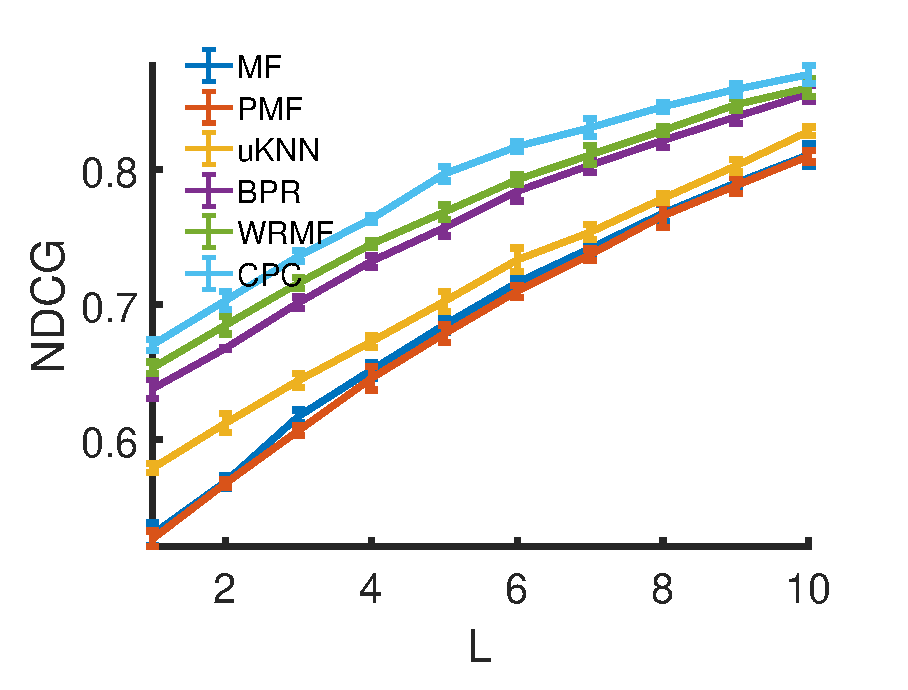
\includegraphics[width=0.23\textwidth]{fig13_compare_NDCG_1.eps}\label{fig:modelNDCG}}
\vspace{-1em}
\hspace{-1em}
\subfigure[CPC v.s. state-of-the-art models]{
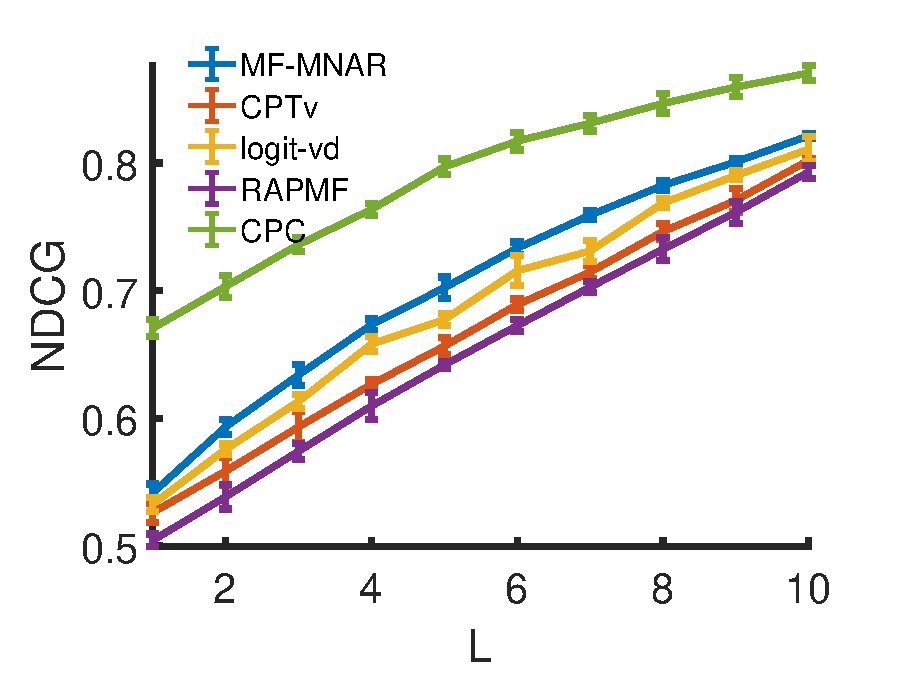
\includegraphics[width=0.23\textwidth]{fig13_compare_NDCG_2.eps}\label{fig:compNDCG}}
\caption{comparable experiment NDCG performance at top L items}
\end{figure}


\subsection{Parameter Tuning}
We have three important parameters in the CPC models $\tau$, $K$ and $C$. In order to see the effects of these parameters, we set $\tau=0.2,0.,5,1.0,1.5,2.0$, $K=5,10,15,20$ and $C=1,2,3,4$. The $NDCG@5$ result of model CPC is shown in Fig.~\ref{fig:parameter}. We can conclude that (1) the performance is quite stable. No matter how we set the parameters,  $NDCG@5>0.74$, which is better than all non-ranking based recommender systems. This again demonstrates the superiority of our models.
(2) The best result is achieved when $\tau=1.5$. It suggests that the hardcore effect is relative strong as $\tau>1$.  (3) $NDCG@5$ results are high for small values of $K,C$. However, when $K$ and $C$ are too large, the performance is harmed due to over-fitting.

\begin{figure*}[htbp]
\centering
\subfigure[$\tau$]{
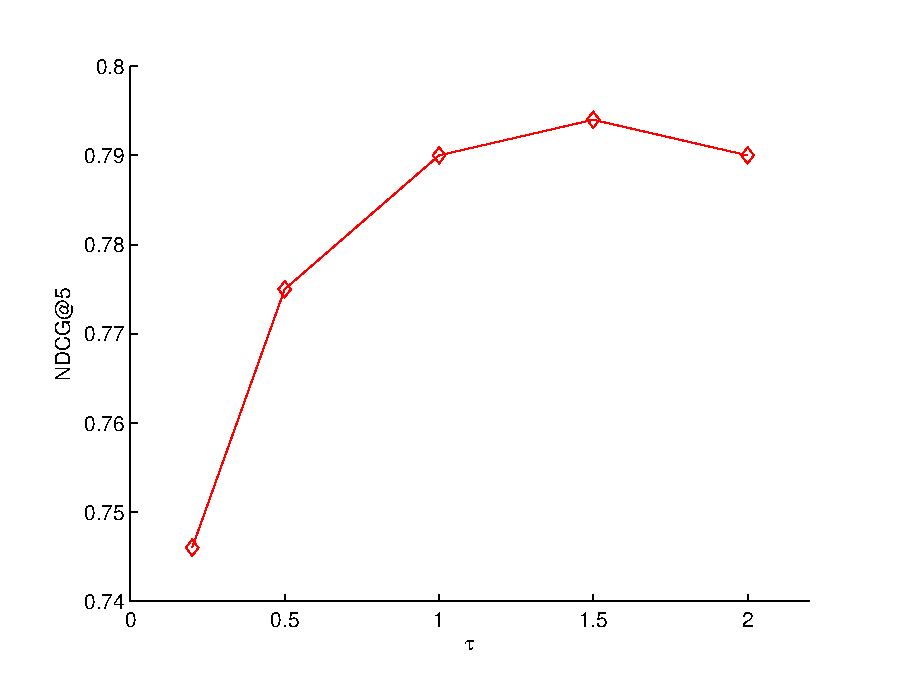
\includegraphics[width=0.2\textwidth]{fig14_tau.eps}}
\subfigure[$K$]{
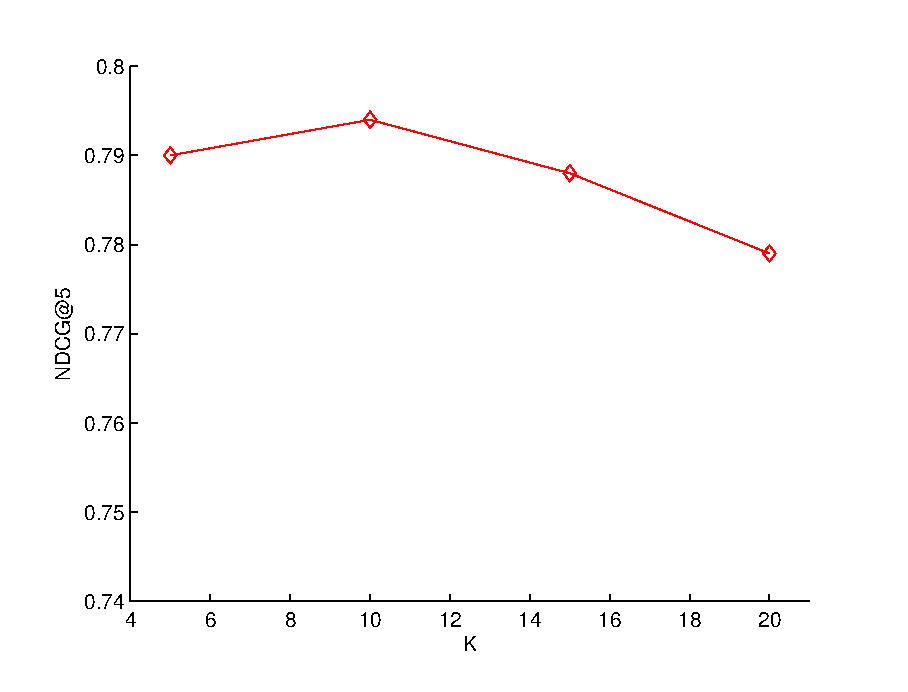
\includegraphics[width=0.2\textwidth]{fig14_k.eps}}
\subfigure[$C$]{
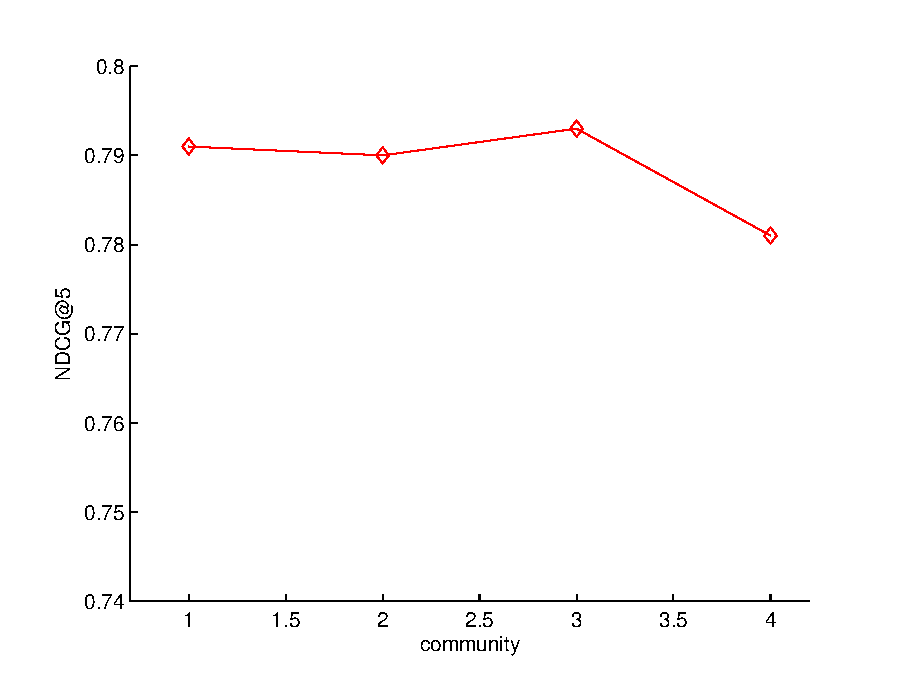
\includegraphics[width=0.2\textwidth]{fig14_C.eps}}
\caption{NDCG@5 performance of CPC over different values of parameters}\label{fig:parameter}
\end{figure*}

\subsection{Perceived Opinion Climate}

In all models, the perceived opinion climate is based on existing ratings. To give a quantitive sense of the necessity to build opinion climate upon observations, we modify Eq.~\ref{equ:ecommunity} as $E_{c,j}=U_cV_j$. In this way, the opinion climate is based on mean user preference within the community.  As shown in Fig.~\ref{fig:umean}, such a modification leads to worse $NDCG@L$ performance at every length $L$ of the recommendation list. It shows that, users need to compare their own opinions to the opinion climate they observed, instead of to the opinion climate they inferred.

\begin{figure}[htbp]
\begin{center}
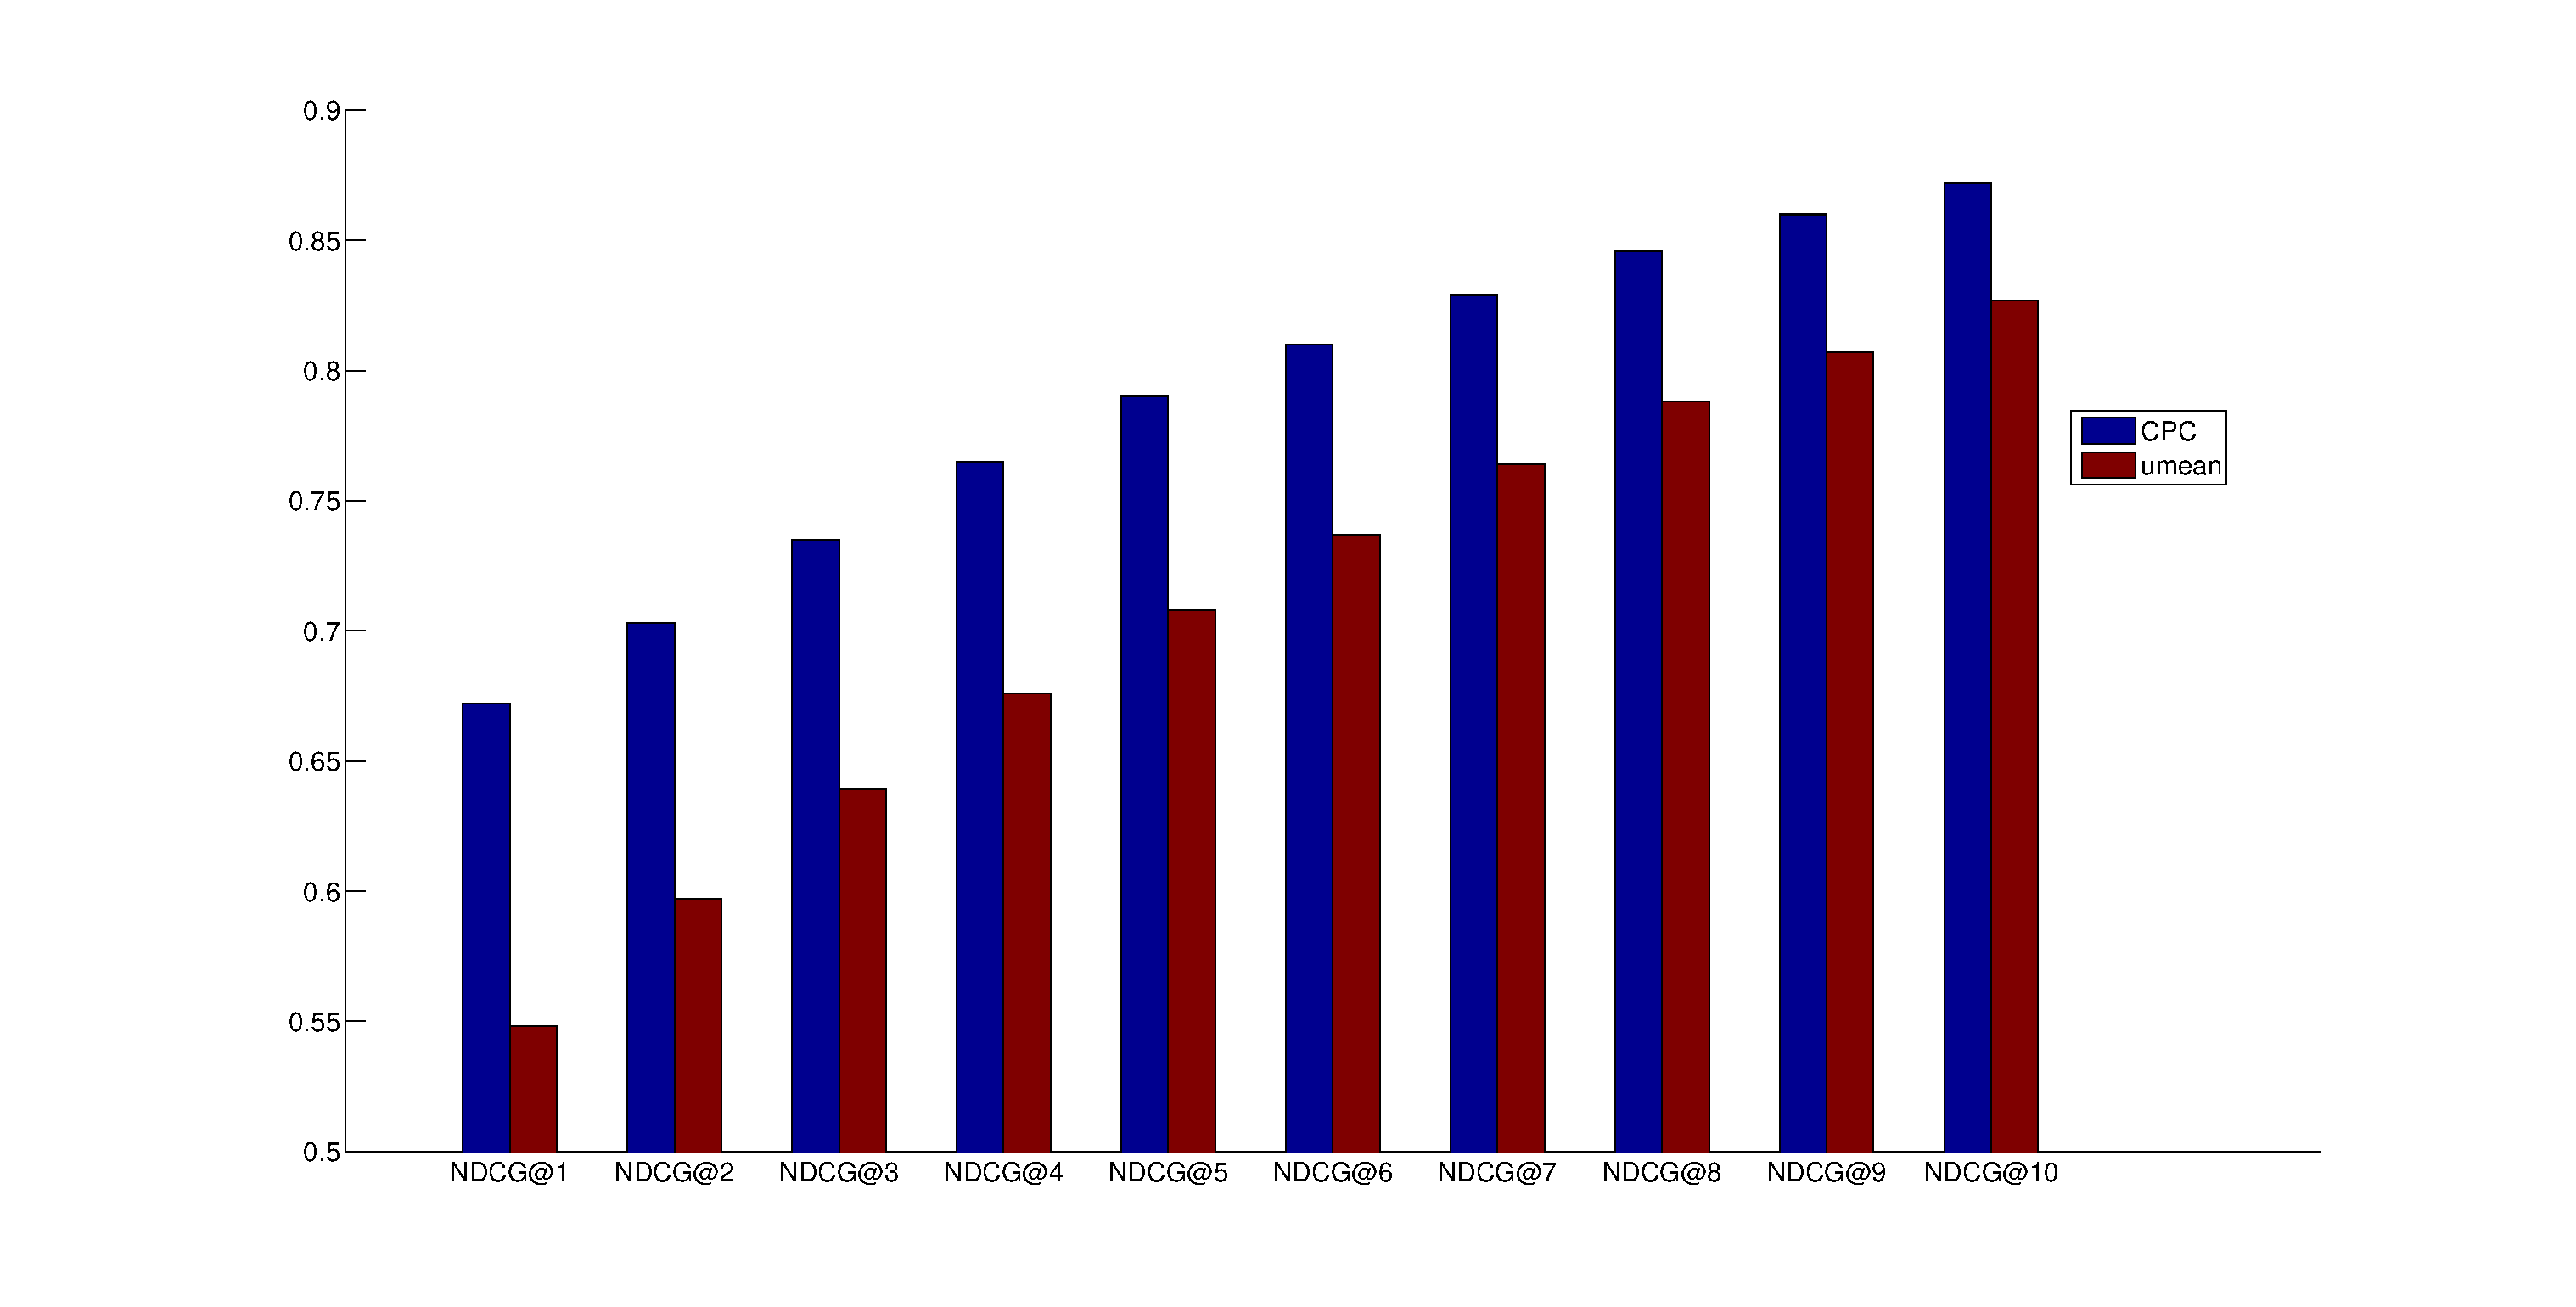
\includegraphics[width=0.45\textwidth]{fig15_umean.eps}
\caption{Performance of CPC on perceived opinion climate and inferred opinion climate}\label{fig:umean}
\label{default}
\end{center}
\end{figure}



\subsection{Supplementary Performance}
Finally, we provide two supplementary experiments. The first one is based on \textbf{A}rea \textbf{U}nder recall-precision \textbf{C}urve (AUC), which is a common measure to evaluate the performance of a binary classifier. We should note that AUC does not reflect how the RS captures MNAR ratings. Therefore, AUC is not the primary measurement for MNAR models. We compare the best performance of our models with parameters $\tau = 1.5, K=10, C=3$ to the state-of-the-art methods in Sec.~\ref{sec:ndcg}.


As shown in Tab.~\ref{tab:AUC}, our models achieve best results in two data sets (Yahoo! and Mtweet). In these two datasets, CPC is significantly better (at significance level $0.01$ and $0.05$) than other models (the significance is tested between the best of our models and the best of other models). CPC achieves second best results in the remaining two data sets (Movielens and Eachmovie). In Eachmovie, the best performing method is not significantly better than our model. Thus our models are at least comparable to the state-of-the art models in term of AUC evaluation. Furthermore, we observe that CPC and COL are comparable when evaluated by AUC.  The underlying reason is that, COL may not be as good as CPC in predicting the top results. But in the long run, the opinion leaders have strong influence over user behaviors. 

\begin{table*}[tbp]
\centering
\caption{Comparative AUC Performances. The best performance is boldfaced. $*,**$ indicates $p\leq 0.05, p\leq 0.01$ based on Wilcoxon signed rank test.}\label{tab:AUC}
\centering
\small
\begin{tabular}{|c|c|c|c|c|c|c|c|c|c|c|c|}
\hline
& Base & CPC & COL & CPP & CPV & uKNN & PMF & CPT-v & logit-vd & MF-MNAR & RAPMF \\\hline
\hline
Yahoo & $0.803$ & $\bf{0.880}**$ & $\bf{0.882}$ & $0.857$ & $0.345$ & $0.776$ & $0.504$ & $0.825$ & $0.841$ & $0.863$ & $0.535$ \\\hline
Mtweet & $0.823$ & $\bf{0.864}*$ & $\bf{0.863}$ & $0.832$ & $0.823$ & $0.766$ & $0.556$ & $0.828$ & $0.832$ & $0.856$ & $0.582$ \\\hline
MovieLen & $0.874$ & $\textbf{0.898}$ & $\bf{0.902}$ & $0.871$ & $0.517$ & $0.818$ & $0.705$ & $0.878$ & $0.882$ & $\bf{0.929}**$ & $0.662$ \\\hline
Eachmovie & $0.840$ & $\bf{0.905}$ & $0.900$ & $0.864$ & $0.776$ & $0.739$ & $0.603$ & $0.792$ & $0.821$ & $\bf{0.912}$ & $0.562$ \\\hline
\end{tabular}
\end{table*}

Another additional evaluation metric is \textbf{U}ser \textbf{C}overage (UC), which is the percentage of all users for which we were able to generate any predictions at all. As MNAR models take responses into account, it is meaningful to evaluate whether the RS can serve all customers, instead of ignoring shy people. For this reason, we only compare our models to other MNAR models. The parameters are  $\tau = 1.5, K=10, C=3$.

As shown in Tab.~\ref{tab:uc}, our models achieve significantly better (at significance level $0.01$ and $0.05$) results in term of UC than other MNAR models in three datasets(the significance is tested between the best of our models and the best of other models). CPC achieves second best result in Movielens, while the best performing method is not significantly better than our model. The UC results demonstrate that our models do not bias towards active users and are able to make accurate predictions for all users.

\begin{table*}[tbp]
\centering
\caption{Comparative UC performances. $*,**$ indicates $p\leq 0.05,p\leq 0.01$ based on Wilcoxon signed rank test.}\label{tab:uc}
\centering
\small
\begin{tabular}{|c|c|c|c|c|c|c|c|c|c|c|}
\hline
Dataset & Base & CPC	& COL&	CPP&	CPV&	CPTv	&logit-vd&	MF-MNAR&	RAPMF\\\hline
\hline
Yahoo	& \textbf{0.0432}* &0.0394 	&\textbf{0.0429}*&	0.0254 &	0.0233 &	0.0318 &	0.0366 	&0.0265 	&0.0132\\\hline 
Mtweet&	\textbf{0.1071}** &0.0569 &	0.0730 	&0.0471 	&0.0413 &	0.0543 &	0.0687 &	0.0695 &	0.0718 \\\hline 
Movielens	&0.1282 & \textbf{0.1329} 	&0.1296 &	0.1155 &	0.1133 &	0.1266 	&\textbf{0.1349} &	0.1177 &	0.0586 \\\hline 
Eachmovie&	0.0924  &\textbf{0.2212}**	&0.2045 &	0.1721 &	0.1819 	&0.1523 	&0.1469& 	0.1943 &	0.0485\\\hline 
 \end{tabular}\label{tab:uc}
\end{table*}

\section{Conclusion}\label{sec:conclusion}

In this contribution we verify the ``spiral of silence'' theory in real recommender systems. We use the empirical discoveries to build recommender models that outperform state-of-the-art recommenders. The proposed models outperform state-of-the-art models in terms of NDCG, AUC and User Coverage. We believe our attempts shed insights into combining social science theories and computational implementations. In the future, we plan to investigate the community detection performance of our CPC model. We would also like to ensemble the four models in different contexts to improve performances.



%\bibliographystyle{abbrv}
%\bibliography{D:/MyRef/MyRef/Reference}

\begin{thebibliography}{10}

\bibitem{Carroll1997Perceived}
J.~G. Carroll, F.~H. Andrew, and J.~Shanahan.
\newblock Perceived support for one's opinions and willingness to speak out: A
  meta-analysis of survey studies on the "spiral of silence".
\newblock {\em The Public Opinion Quarterly}, 61(3):452--463, 1997.

\bibitem{Cohen1970dissonance}
J.~B. Cohen and M.~E. Goldberg.
\newblock The dissonance model in post-decision product evaluation.
\newblock {\em Journal of Marketing Research}, pages 315--321, 1970.

\bibitem{Dalvi2013Para}
N.~N. Dalvi, R.~Kumar, and B.~Pang.
\newblock Para 'normal' activity: On the distribution of average ratings.
\newblock In {\em (ICWSM)}, pages 110--119, 2013.

\bibitem{Godes2012Sequential}
D.~Godes and J.~C. Silva.
\newblock Sequential and temporal dynamics of online opinion.
\newblock {\em Marketing Science}, 31(3):448--473, 2012.

\bibitem{Gopalan2015Scalable}
P.~Gopalan, J.~Hofman, and D.~Blei.
\newblock Scalable recommendation with hierarchical poisson factorization.
\newblock In {\em UAI},
  2015.

\bibitem{Hernandez-Lobato2014Probabilistic}
J.~M. Hernandez-Lobato, N.~Houlsby, and Z.~Ghahramani.
\newblock Probabilistic matrix factorization with non-random missing data.
\newblock In {\em ICML}, 2014.

\bibitem{Hu2009Overcoming}
N.~Hu, J.~Zhang, and P.~A. Pavlou.
\newblock Overcoming the j-shaped distribution of product reviews.
\newblock {\em Commun. ACM}, 52(10):144--147, Oct. 2009.

\bibitem{Jamali2011Generalized}
M.~Jamali, T.~Huang, and M.~Ester.
\newblock A generalized stochastic block model for recommendation in social
  rating networks.
\newblock In {\em RecSys } 2011, pages 53--60.

\bibitem{Jindal2008Opinion}
N.~Jindal and B.~Liu.
\newblock Opinion spam and analysis.
\newblock In {\em  WSDM} 2008, pages 219--230.

\bibitem{Kennamer1990Self}
J.~D. Kennamer.
\newblock Self-serving bibias in perceiving the opinions of others.
\newblock {\em Communication Research}, 17:393--404, 1990.

\bibitem{Kim2014Bayesian}
Y.-D. Kim and S.~Choi.
\newblock Bayesian binomial mixture model for collaborative prediction with
  non-random missing data.
\newblock In {\em  RecSys } 2014, pages 201--208.

\bibitem{Koren2009Matrix}
Y.~Koren, R.~Bell, and C.~Volinsky.
\newblock Matrix factorization techniques for recommender systems.
\newblock {\em Computer}, 42(8):30--37, 2009.

\bibitem{Liang2016Modeling}
D.~Liang, L.~Charlin, J.~McInerney, and D.~M. Blei.
\newblock Modeling user exposure in recommendation.
\newblock In {\em WWW } 2016, pages 951--961.

\bibitem{Ling2012Response}
G.~Ling, H.~Yang, M.~R. Lyu, and I.~King.
\newblock Response aware model-based collaborative filtering.
\newblock In {\em UAI}, pages 501--510, 2012.

\bibitem{Liu2011Wisdom}
N.~N. Liu, X.~Meng, C.~Liu, and Q.~Yang.
\newblock Wisdom of the better few: Cold start recommendation via
  representative based rating elicitation.
\newblock In {\em  RecSys } 2011, pages 37--44.

\bibitem{Marlin2009Collaborative}
B.~M. Marlin and R.~S. Zemel.
\newblock Collaborative prediction and ranking with non-random missing data.
\newblock In {\em RecSys}  2009, pages 5--12.

\bibitem{mcdevitt2003spiral}
M.~McDevitt, S.~Kiousis, and K.~Wahl-Jorgensen.
\newblock Spiral of moderation: Opinion expression in computer-mediated
  discussion.
\newblock {\em International Journal of Public Opinion Research},
  15(4):454--470, 2003.

\bibitem{Neolle-Neumann1993spiral}
E.~Neolle-Neumann.
\newblock {\em The spiral of silence: Public opinion, our social skin.}
\newblock University of Chicago Press., 1993.

\bibitem{Ohsawa2016Gated}
S.~Ohsawa, Y.~Obara, and T.~Osogami.
\newblock Gated probabilistic matrix factorization: Learning users鈥?attention
  from missing values.
\newblock In {\em IJCAI}, pages 1888--1894, 2016.

\bibitem{Pradel2012Ranking}
B.~Pradel, N.~Usunier, and P.~Gallinari.
\newblock Ranking with non-random missing ratings: Influence of popularity and
  positivity on evaluation metrics.
\newblock In {\em RecSys } 2012, pages 147--154.

\bibitem{salakhutdinov2008probabilistic}
R.~Salakhutdinov and A.~Mnih.
\newblock Probabilistic matrix factorization.
\newblock {\em NIPS},
  20:1257--1264, 2008.

\bibitem{Steck2010Training}
H.~Steck.
\newblock Training and testing of recommender systems on data missing not at
  random.
\newblock In {\em SIGKDD } 2010, pages 713--722.

\bibitem{Yang2015Boosting}
H.~Yang, G.~Ling, Y.~Su, M.~R. Lyu, and I.~King.
\newblock Boosting response aware model-based collaborative filtering.
\newblock {\em IEEE Transactions on Knowledge and Data Engineering},
  27(8):2064--2077, Aug 2015.
  
\bibitem{Rendle2009BPR}
 Rendle, S.; Freudenthaler, C.; Gantner, Z. and Schmidt-Thieme, L. 
 \newblock BPR: Bayesian Personalized Ranking from Implicit Feedback 
 \newblock In {\em UAI}, 2009, 452-461
 
\bibitem{Liu2016Are}
Liu, Y, Cao, X. and Yu, Y. 
\newblock Are You Influenced by Others When Rating?: Improve Rating Prediction by Conformity Modeling 
\newblock In {\em RecSys}, 2016, 269-272

\end{thebibliography}

%\balancecolumns
\end{document}
